%% 该模板修改自《计算机学报》latex 模板
%% 主要是将双栏改成单栏,去掉了部分计算机学报标识;
%% 源文件自:https://www.overleaf.com/latex/templates/latextemplet-cjc-xelatex/ybmmymncrrmw
%% 
%%
%% This is file `CjC_template_tex.tex',
%% is modified by Zhi Wang (zhiwang@ieee.org) based on the template 
%% provided by Chinese Journal of Computers (http://cjc.ict.ac.cn/).
%%
%% This version is capable with Overleaf (XeLaTeX).
%%
%% Update date: 2023/03/10
%% -------------------------------------------------------------------
%% Copyright (C) 2016--2023 
%% -------------------------------------------------------------------
%% This file may be distributed and/or modified under the
%% conditions of the LaTeX Project Public License, either version 1.3c
%% of this license or (at your option) any later version.
%% The latest version of this license is in
%%    https://www.latex-project.org/lppl.txt
%% and version 1.3c or later is part of all distributions of LaTeX
%% version 2008 or later.
%% -------------------------------------------------------------------

\documentclass[10.5pt,compsoc,UTF8]{CjC}
\usepackage{CTEX}
\usepackage{graphicx}
\usepackage{footmisc}
\usepackage{subfigure}
\usepackage{url}
\usepackage{multirow}
\usepackage{multicol}
\usepackage[noadjust]{cite}
\usepackage{amsmath,amsthm}
\usepackage{amssymb,amsfonts}
\usepackage{booktabs}
\usepackage{color}
\usepackage{ccaption}
\usepackage{booktabs}
\usepackage{float}
\usepackage{fancyhdr}
\usepackage{caption}
\usepackage{xcolor,stfloats}
\usepackage{comment}
\setcounter{page}{1}
\graphicspath{{figures/}}
\usepackage{cuted}%flushend,
\usepackage{captionhack}
\usepackage{epstopdf}
\usepackage{gbt7714}
\usepackage{listings}
\usepackage{xeCJK}
\usepackage{float}
\usepackage{sourcecodepro}
\usepackage[T1]{fontenc}
\usepackage{hyperref}

\setmainfont{Times Roman}
% \setCJKmainfont{Noto Sans Mono CJK TC}
\setCJKmainfont{標楷體.ttc}
\setmonofont{Cascadia Code}

%===============================%

\headevenname{\mbox{\quad} \hfill  \mbox{\zihao{-5}{ \hfill 2024 Hardware Design  } \hspace {50mm} \mbox{2024 年 10 月}}}%
\headoddname{Group 21 \hfill Lab 3: Sequential-Circuits}%

%footnote use of *
\renewcommand{\thefootnote}{\fnsymbol{footnote}}
\setcounter{footnote}{0}
\renewcommand\footnotelayout{\zihao{5-}}

\newtheoremstyle{mystyle}{0pt}{0pt}{\normalfont}{1em}{\bf}{}{1em}{}
\theoremstyle{mystyle}
\renewcommand\figurename{figure~}
\renewcommand{\thesubfigure}{(\alph{subfigure})}
\newcommand{\upcite}[1]{\textsuperscript{\cite{#1}}}
\renewcommand{\labelenumi}{(\arabic{enumi})}
\newcommand{\tabincell}[2]{\begin{tabular}{@{}#1@{}}#2\end{tabular}}
\newcommand{\abc}{\color{white}\vrule width 2pt}
\renewcommand{\bibsection}{}
\makeatletter
\renewcommand{\@biblabel}[1]{[#1]\hfill}
\makeatother
\setlength\parindent{2em}
%\renewcommand{\hth}{\begin{CJK*}{UTF8}{gbsn}}
%\renewcommand{\htss}{\begin{CJK*}{UTF8}{gbsn}}
\renewcommand{\contentsname}{Table of Contents}

\begin{document}

\hyphenpenalty=50000
\makeatletter
\newcommand\mysmall{\@setfontsize\mysmall{7}{9.5}}
\newenvironment{tablehere}
  {\def\@captype{table}}

\let\temp\footnote
\renewcommand \footnote[1]{\temp{\zihao{-5}#1}}

\hypersetup{
  colorlinks=false,
  pdfborder={0 0 0},
}

\thispagestyle{plain}%
\thispagestyle{empty}%
\pagestyle{CjCheadings}

% \begin{table*}[!t]
\vspace {-13mm}


\onecolumn
\zihao{5-}\noindent Group 21 \hfill Lab 3: Sequential-Circuits \hfill 2024 年 10 月\\
\noindent\rule[0.25\baselineskip]{\textwidth}{1pt}


\begin{center}
    \vspace {11mm}
    {\zihao{2} \heiti \fangsong Lab 3: Sequential-Circuits }
    
    \vskip 5mm
    
    {\zihao{4}\fangsong Group 21: 陳克盈(112062205)、蔡明妡(112062224)}
\end{center}

\lstset{
    % backgroundcolor=\color{red!50!green!50!blue!50},%程式碼塊背景色為淺灰色
    rulesepcolor= \color{gray}, %程式碼塊邊框顏色
    breaklines=true,  %程式碼過長則換行
    numbers=left, %行號在左側顯示
    numberstyle= \small\ttfamily,%行號字型
    keywordstyle= \color{blue},%關鍵字顏色
    commentstyle=\color{gray}, %註釋顏色
    frame=shadowbox%用方框框住程式碼塊
    basicstyle=\ttfamily\footnotesize,
}
 
\definecolor{improvecolor}{rgb}{0,0.6,0} % 深綠色
\definecolor{declinecolor}{rgb}{0.6,0,0} % 深紅色


%%%%%%%%%%%%%%%%%%%%%%%%%%%%%%%%%%%%%%
\zihao{5}
\vskip 10mm
% \begin{multicols}{1}


%%%%%%%%%%%%%%%%%%%%%%%%%%%%%%%%%%%%%%%%%%
%%%%%%%%%%%%%%%%%%%%%%%%%%%%%%%%%%%%%%%%%%

\tableofcontents
\newpage

\section{Q1: 4-bit Ping-Pong Counter}
\label{sec:Q1}

\subsection{Implement}
這題需要實作一個 4-bit 的 Ping-Pong Counter,會從 0 開始累加\
,直到 15 後再從 15 開始減少至 0,不斷循環。

在 verilog 程式碼方面,我們使用了多個 if 條件式,判斷目前屬於什麼狀態:
\begin{itemize}
  \item $rst\_n = 0$: 將 $started, direction$ 設為 true, 並將輸出 $out$ 設為 $0$。
  \item $started \& enable$:代表 Counter 正在運作,此時會根據 $direction$ 進行加減:
  \begin{itemize}
    \item $out = 15, direction = 1$:代表再繼續往上就會超出範圍,因此將 $direction$ 設為 $0$ 並將輸出 $-1$
    \item $out = 0, direction = 0$:與上個情況相反,將 $direction$ 設為 $1$ 並將輸出 $+1$
    \item 其他情況:根據 $direction$ 進行加減
  \end{itemize}
\end{itemize}

\subsection{Circuit}

在電路方面,需要實作的部分如下:
\begin{itemize}
  \item $started, direction, out$ 儲存:使用了三個 D-Flip-Flop 來儲存
  \item 計算下一個 clock cycle 的 $out, direction$:每個 clock cycle 會根據當下的 $out, direction$,透過加減法器預先算出 $out + 1, out - 1$,\
  再透過多個 AND gate, NOT Gate,來實作出上述的條件式,分別導至四條線路。\
  最後,再利用 MUX,根據對應的線路與條件來決定下一個 clock cycle 的 $out$ 以及 $direction$。
  \item enable:算出 $out, direction$ 之後,利用 MUX 處理 $enable$,若是 $enable = True$,則將 新的 $out, direction$ 輸入至 D-Flip-Flop,\
  否則就輸入原來的值。
  \item reset:在上述訊號都處理完後,會再經過一關判斷是否需要 reset,如果不用則使用上述計算出來的值,否則就將該值設為初始值。
\end{itemize}

\newpage

\begin{figure}[!h]
  \centering
  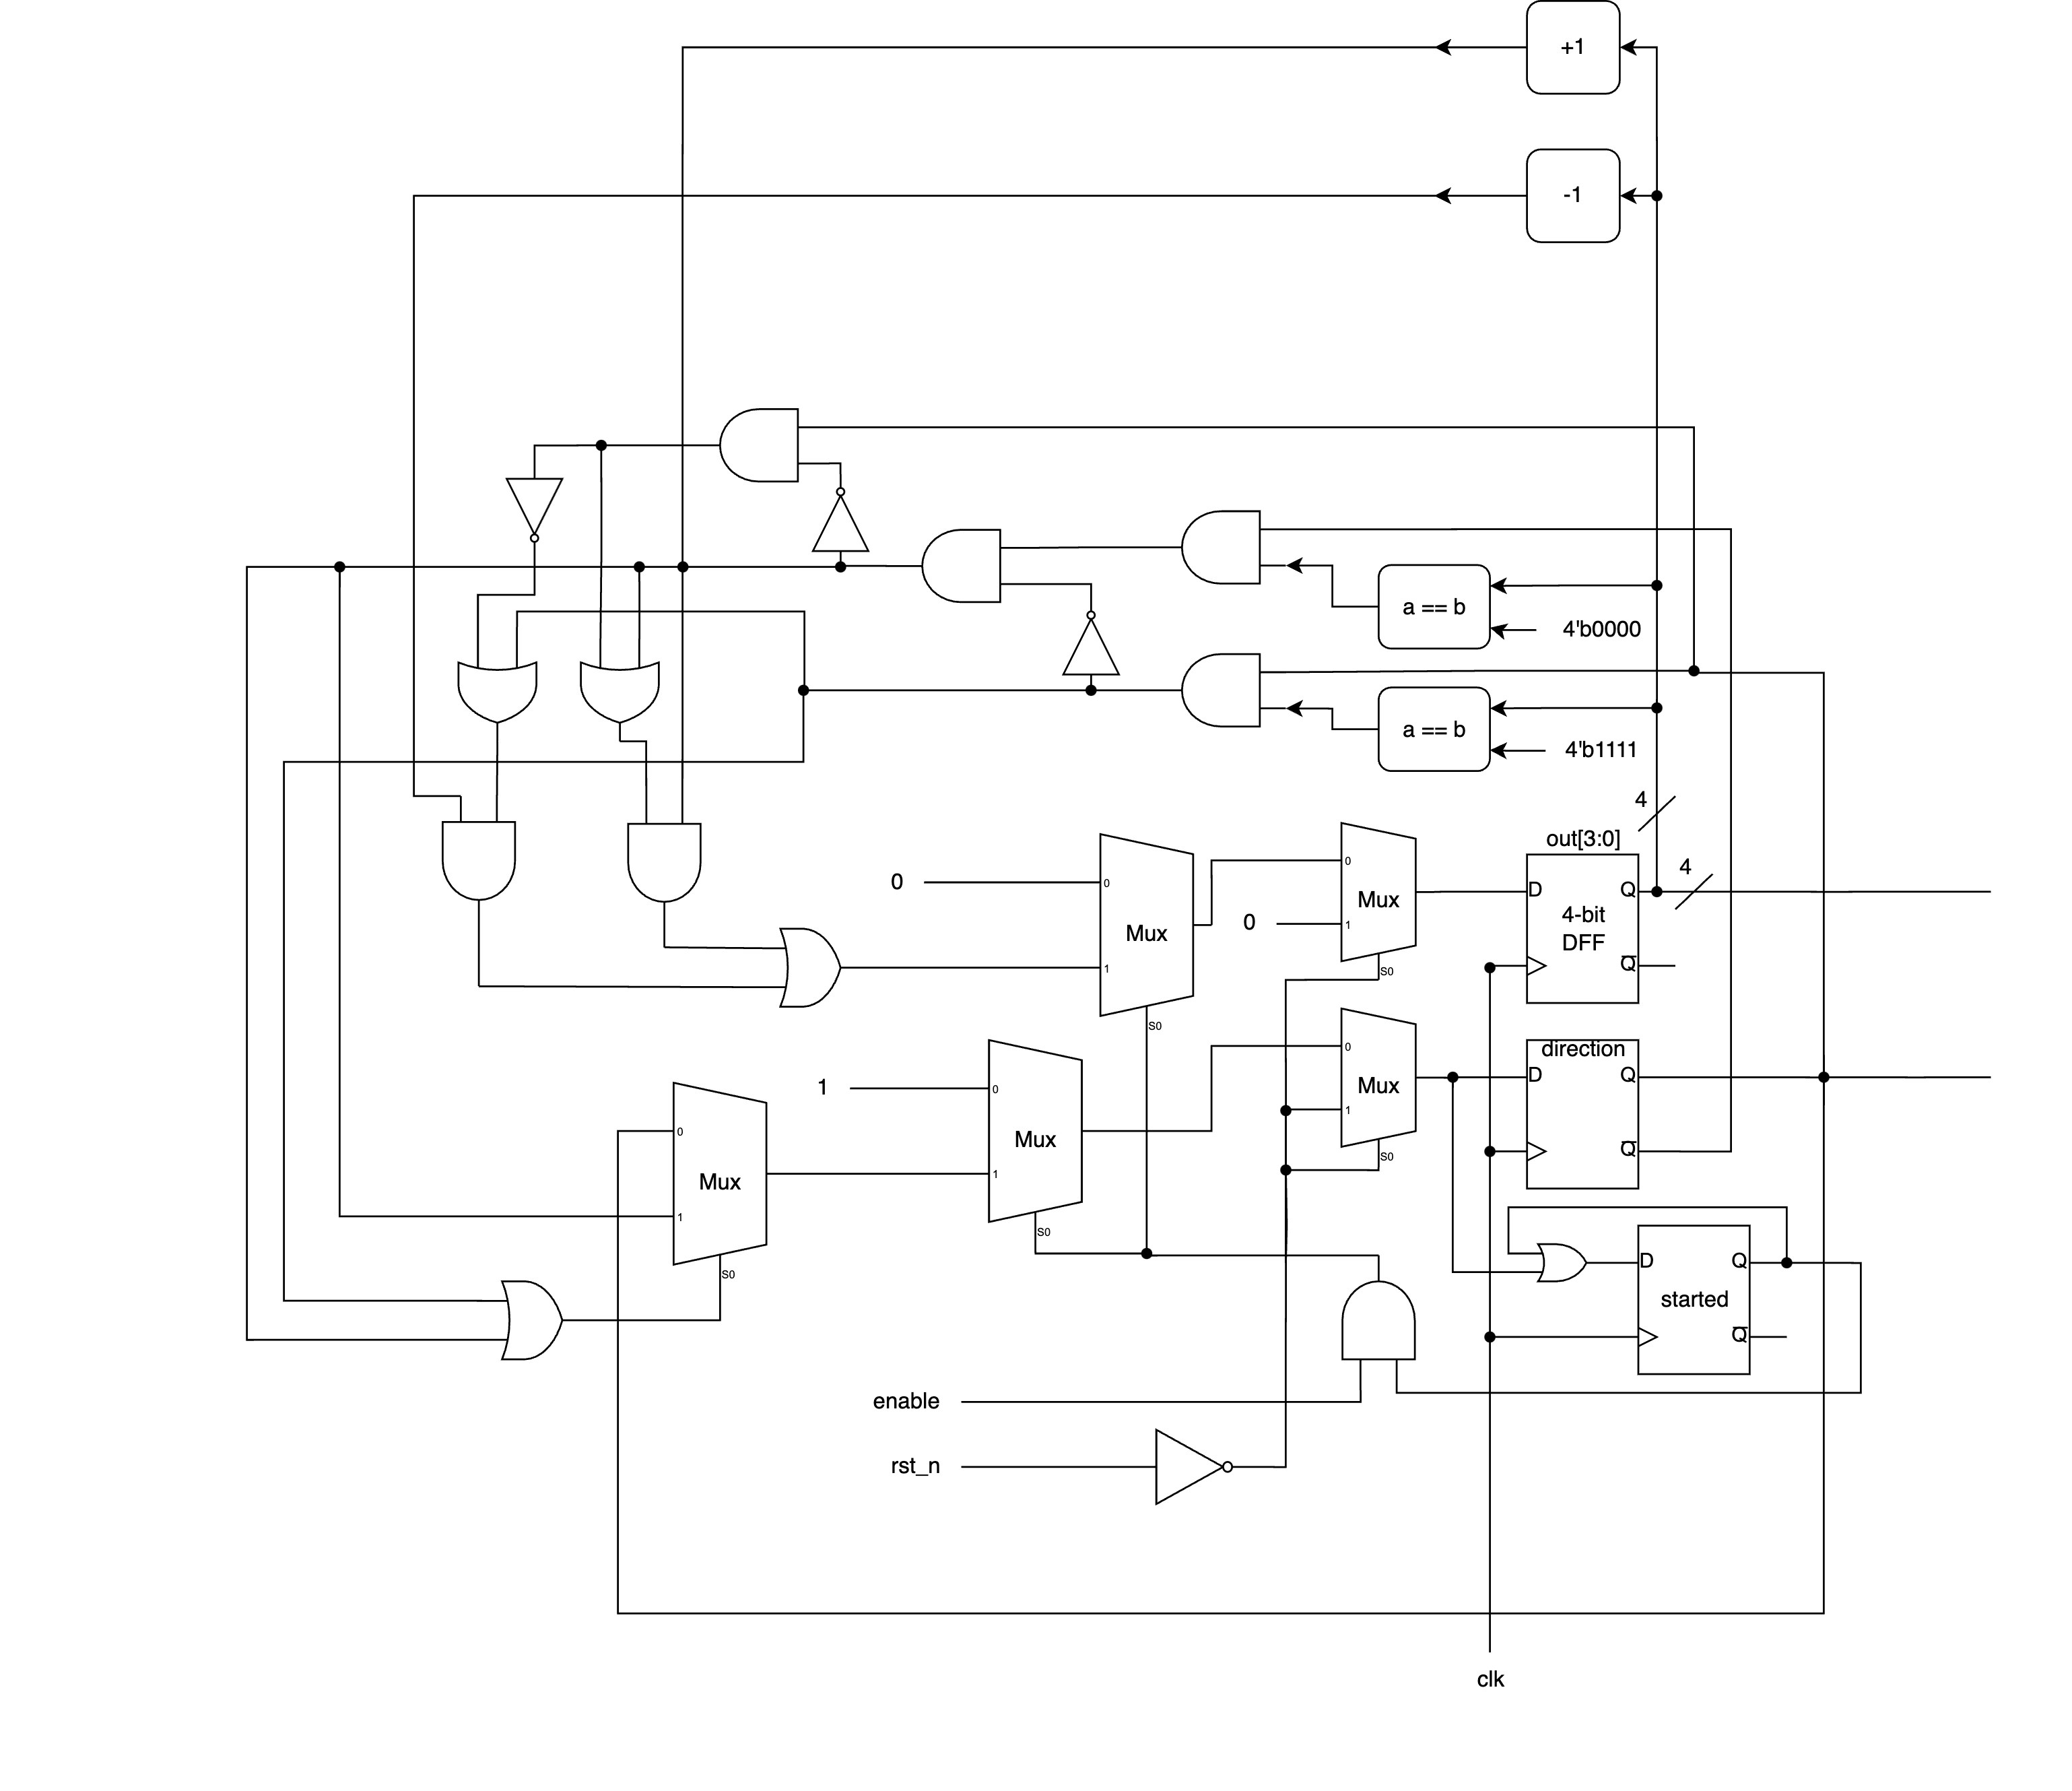
\includegraphics[width=\textwidth]{./img/Q1.png}
  \caption{Q1 Circuit}
  \label{fig:Q1}
\end{figure}

\newpage

\subsection{Testbench}
由於操作相較單純,因此直接利用一個迴圈跑 $2^8$ 次,每次都將 enable 反轉,觀察輸出是否符合預期:

\begin{figure}[!h]
  \centering
  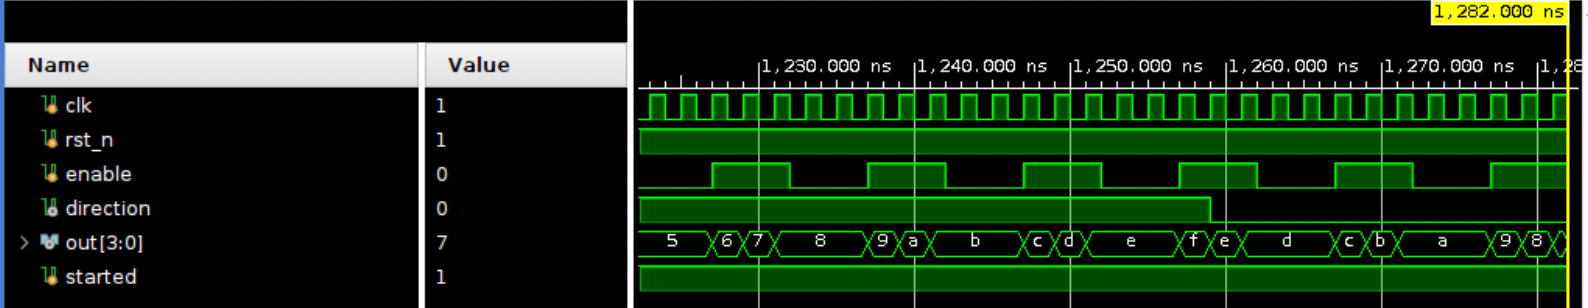
\includegraphics[width=\textwidth]{./img/Q1-tb-wave1.png}
  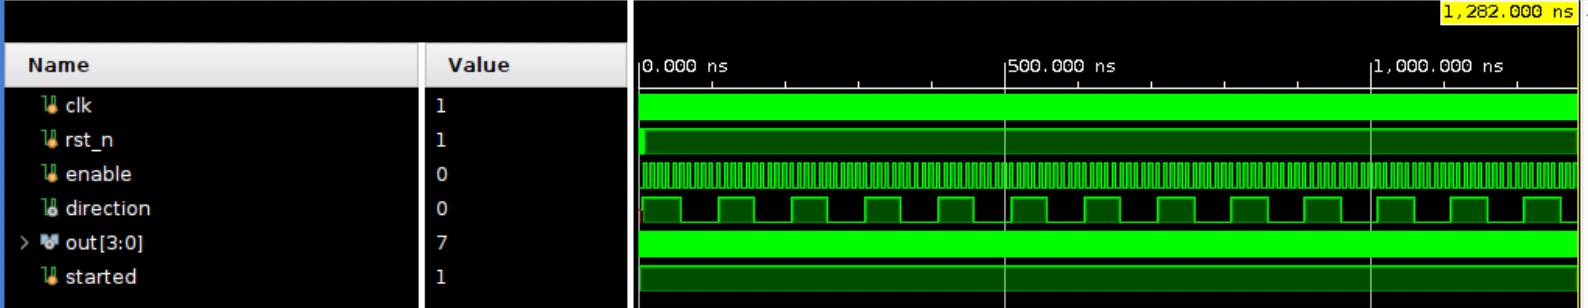
\includegraphics[width=\textwidth]{./img/Q1-tb-wave2.png}
  \caption{Q1 Testbench Wave}
  \label{fig:Q1-tb}
\end{figure}

\section{Q2: First-In First Out (FIFO) Queue}
\label{sec:Q2}

\subsection{Implement \& Circuit}

這邊要實現一個 8 個 8-bit 資料的 Queue (First in First out),\
實作內容主要以這幾個數值的計算為主:
\begin{itemize}
  \item $started$:是否開始運作,為 register,會在每個 posedge 時被計算
  \item $raddr$:讀取的位址,為 register,會在每個 posedge 時被計算
  \item $waddr$:下一次要寫入的位址,為 register,會在每個 posedge 時被計算
  \item $count$:目前 Queue 中有幾個資料,為 register,會在每個 posedge 時被計算
  \item $error$:是否有錯誤,為 wire,判斷方式為:\
  當 $count = 0$ 且 $ren = 0$,或是 $count = 8$ 且 $wen = 1$ 時,error 為 True,\
  前者代表沒有資料可以讀取,後者代表沒有空間可以寫入。
\end{itemize}

而操作過程如下:
\begin{enumerate}
  \item reset:當 $rst\_n$ 與 $started$ 皆為 False 時,將 $started$ 設為 True
  \item 開始後,如果沒有錯誤且 $ren = 1$,則將輸出設定為 $raddr$ 的位置、將 $raddr$ 設為 $raddr + 1$,\
  以及將 $count$ 減一
  \item 如果上述條件都沒有達到,且要寫入的話,則將 $waddr$ 的位置設定為 $din$ (data input)、\
  將 $waddr$ 設為 $waddr + 1$,以及將 $count$ 加一
\end{enumerate}

\newpage

\subsubsection*{Memory}
首先先介紹我們設計的記憶體單位,我們透過 8 個 8-bit 的 D-Flip-Flop 作為儲存單位,\ 
而記憶體控制的部分,除了 clock 之外會接收 4 個參數,分別為:
\begin{itemize}
  \item $ren$:是否讀取記憶體
  \item $wen$:是否寫入記憶體
  \item $addr$:讀取或寫入的記憶體位置
  \item $din$:寫入的資料
\end{itemize}
並且會輸出 $dout$,代表讀取的資料。
\par
判斷邏輯會是這樣的步驟:
\begin{enumerate}
  \item 如果 $ren = 1$,那麼不執行寫入,直接輸出 $addr$ 這個位置的值
  \item 如果沒有要讀取,且要寫入的話,那麼就將 $din$ 的值設為是 $addr$ 這個位置新的值
  \item 沒有要讀取也沒有要寫入的話,就輸出 $0$ 然後不對 DFF 做任何動作
\end{enumerate}

在電路實現的部分,大致會分成幾層:
\begin{enumerate}
  \item 判斷輸入:首先使用比較器對每個位址 $i$ 判斷 $addr$ 是否等於 $i$,\
  並將其結果與 $!ren \& wen$ 做 AND,得到的結果便是這個位址是否要寫入。
  \item D-Flip-Flop 控制:在每個 DFF 前加上一個 MUX,根據上述的結果決定 DFF 的輸入是\
  $din$ 還是原本的值
  \item 輸出判斷:與第一步相似但相較簡單,直接使用比較器判斷 $addr$ 是否等於 $i$,\
  並將結果與 DFF 的輸出做 AND,就能得到這個位址的輸出值。由於只會有一個位址會有輸出值,\
  因此在最後直接做 Bitwise OR 就可以得到最終的輸出。
\end{enumerate}

下圖演示的是 8 個 8-bit 的記憶體,可根據需求調整每個單位的位元大小以及有幾個單位。
\newpage

\begin{figure}[!h]
  \centering
  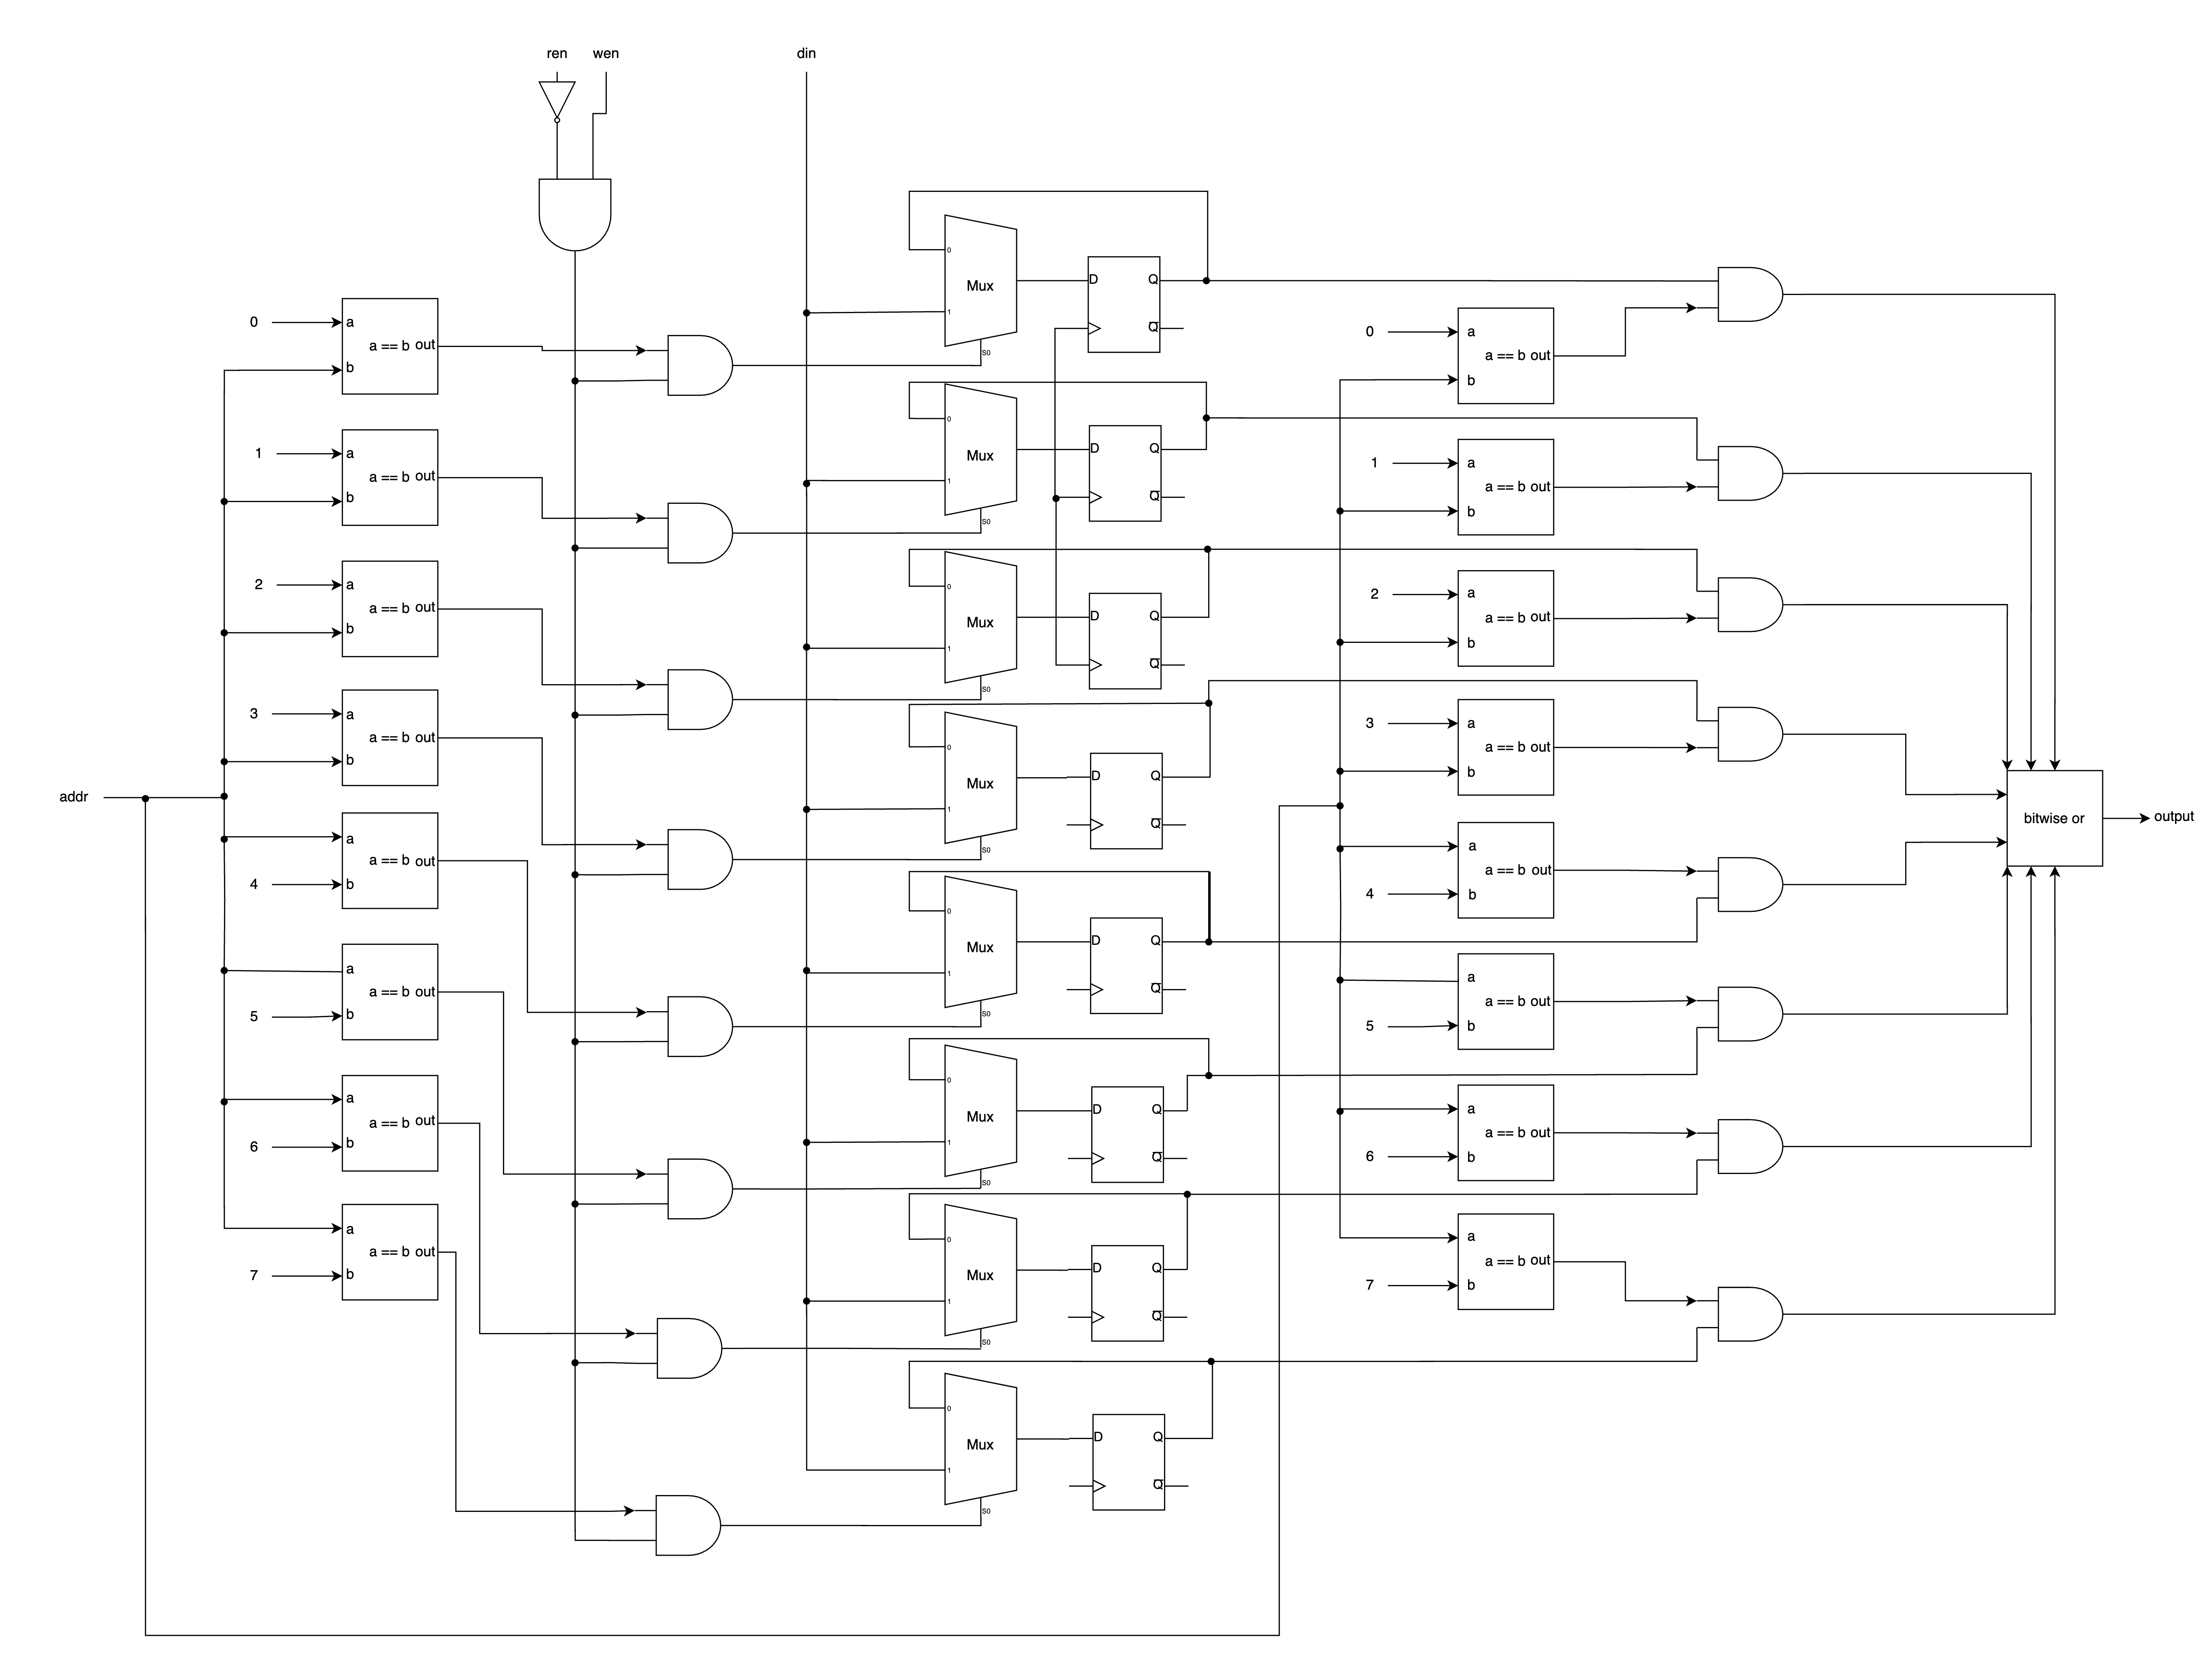
\includegraphics[width=\textwidth]{./img/Memory.png}
  \caption{Memory}
  \label{fig:Memory}
\end{figure}
\newpage

\subsubsection*{FIFO}
FIFO 的部分則是利用了上述的記憶體單位,計算出要傳給 Memory 的 $ren, wen, addr, din$ 後,得到輸出的結果。

\begin{figure}[!h]
  \centering
  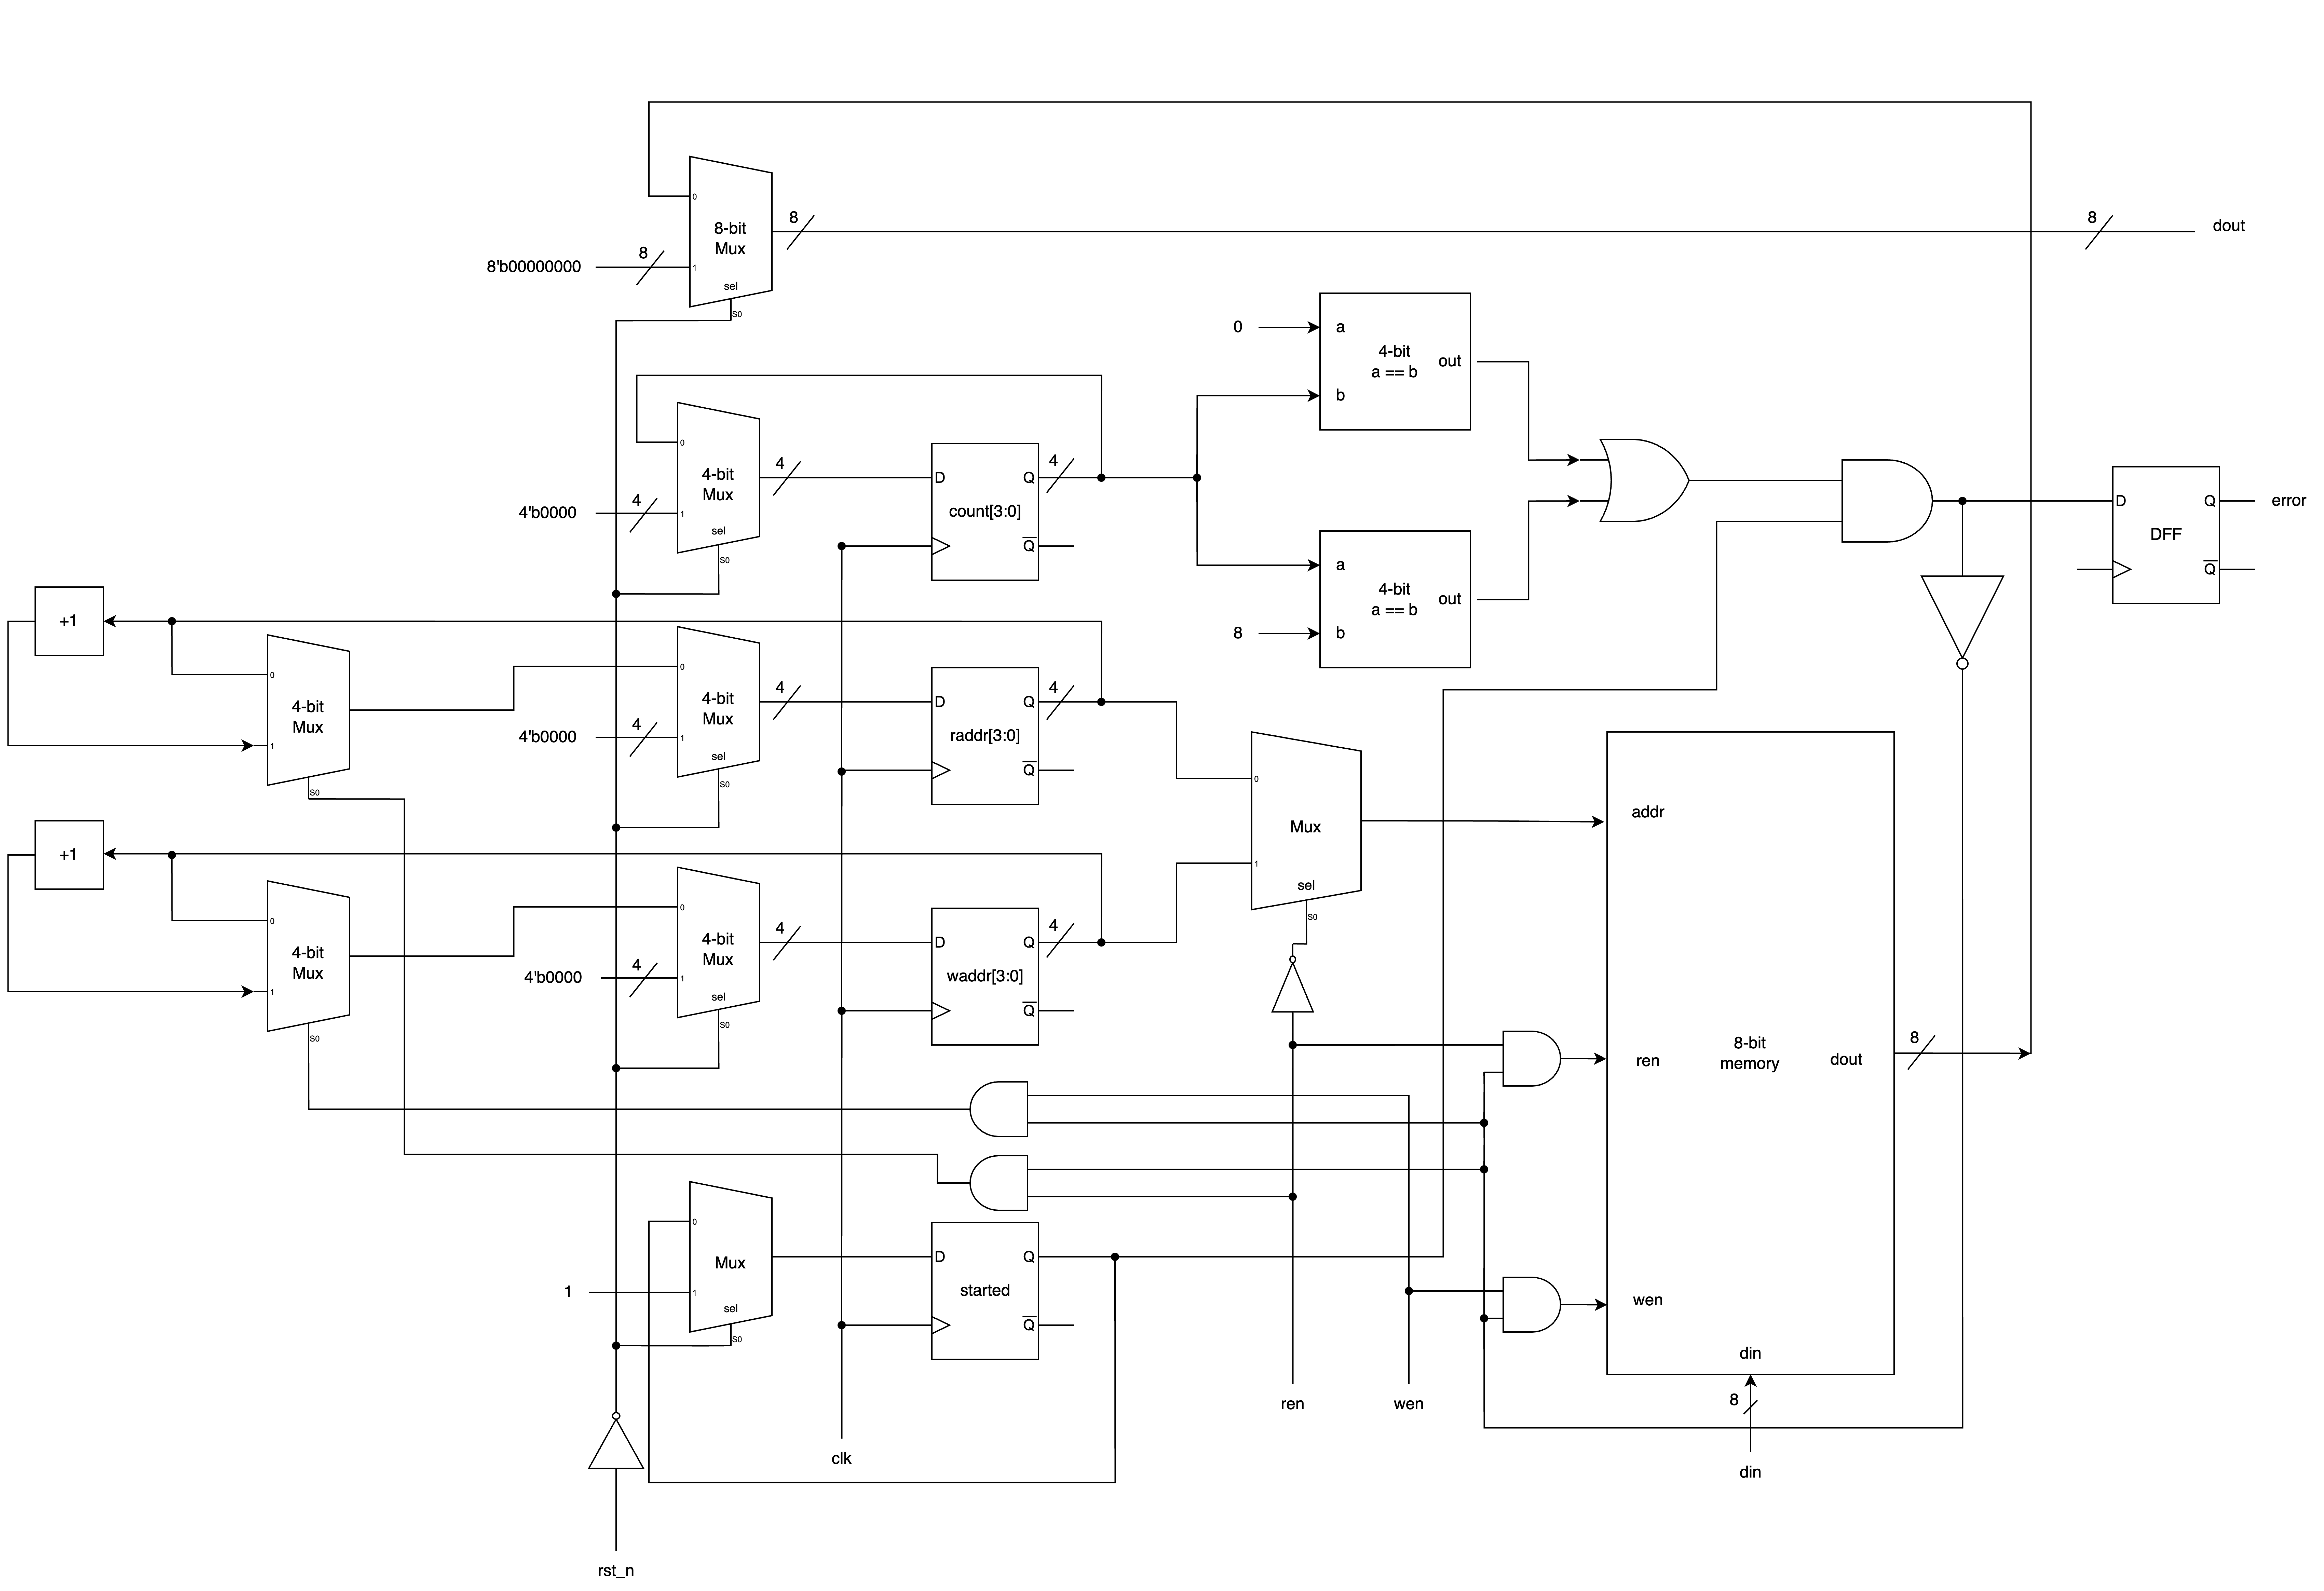
\includegraphics[width=\textwidth]{./img/Q2.png}
  \caption{Q2 Circuit}
  \label{fig:Q2-Circuit}
\end{figure}

\subsection{Testbench}
我們寫了兩個 Testbench,首先是重現題目範例中的波形圖:

\begin{figure}[!h]
  \centering
  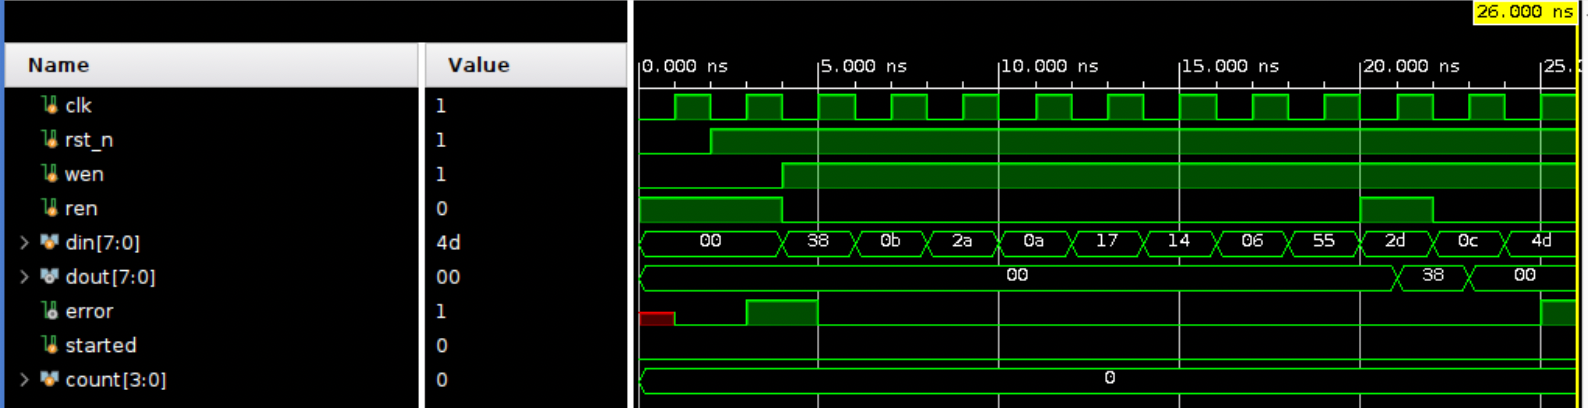
\includegraphics[width=\textwidth]{./img/Q2-tb-ex.png}
  \caption{Q2 Example Testbench}
  \label{fig:Q2-tb-ex}
\end{figure}

\newpage

接著是我們使用 SystemVerilog 提供的 Queue,進行更完整的測試。\
由於 $ren, wen, din$ 的組合數太多,因此我選擇了使用跑 $2^{10}$ 測試,每次將這些輸入值設定為一個隨機值,\
藉此來跑到盡可能多的 case,並透過與 SystemVerilog 中,絕對正確的 Queue 來比對是否有錯誤。\
執行結果如圖 \ref{fig:Q2-tb-sv} 所示。

\begin{figure}[!h]
  \centering
  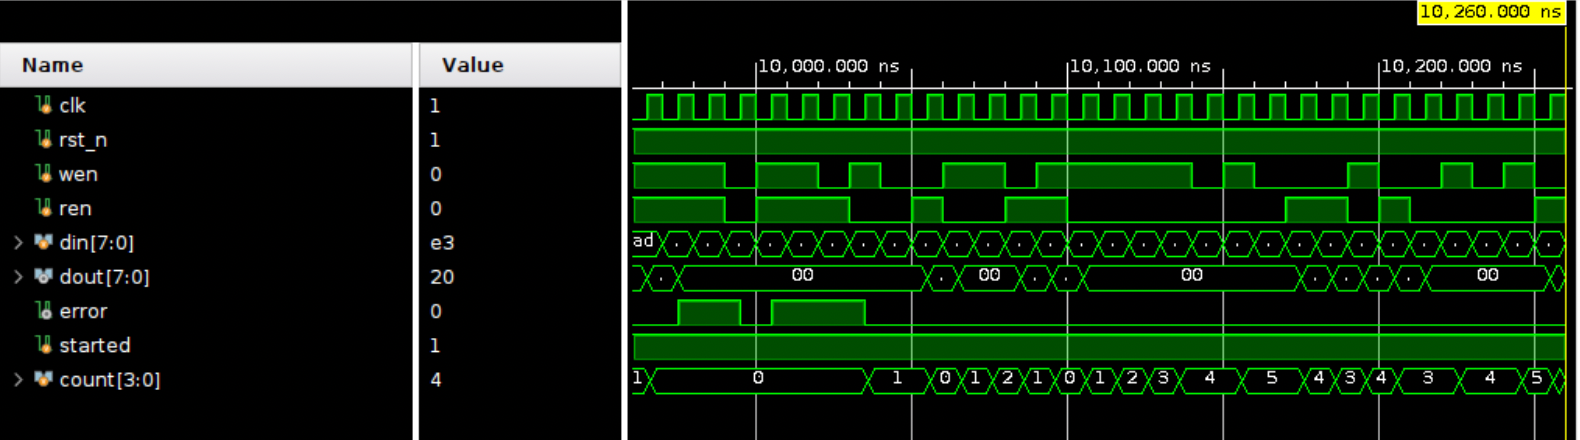
\includegraphics[width=0.9\textwidth]{./img/Q2-tb-sv-wave1.png}
  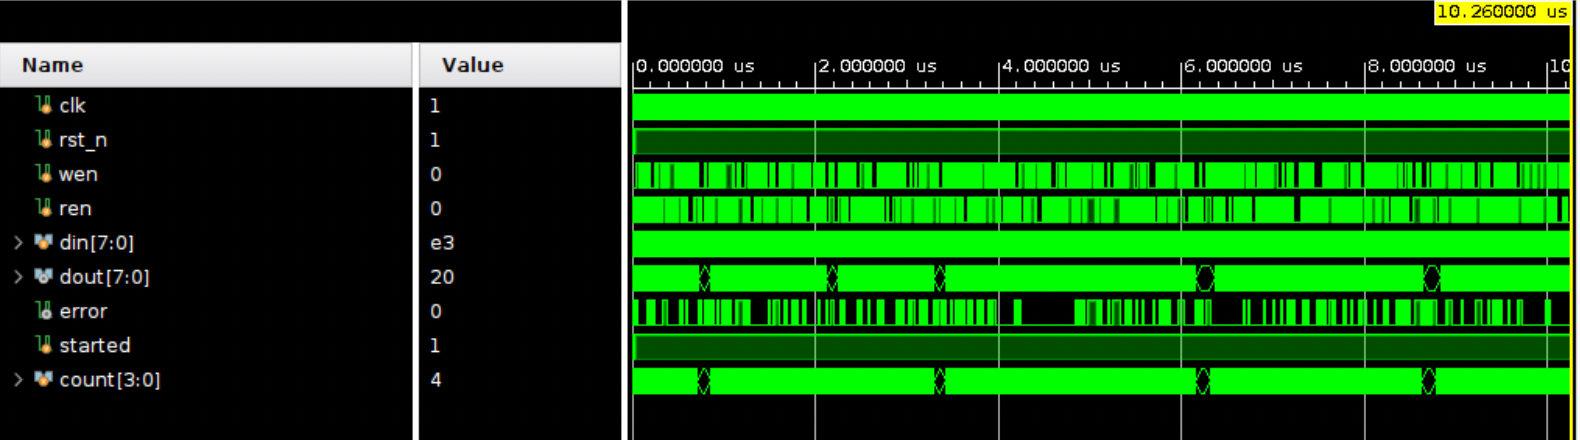
\includegraphics[width=0.9\textwidth]{./img/Q2-tb-sv-wave2.png}
  \caption{Q2 SystemVerilog Testbench Wave}
  \label{fig:Q2-tb-sv}
\end{figure}

但由於 NTHUCAD 不支援 SystemVerilog,因此額外再寫了一個 Testbench。執行結果如下圖 \ref{fig:Q2-tb} 所示。

\begin{figure}[!h]
  \centering
  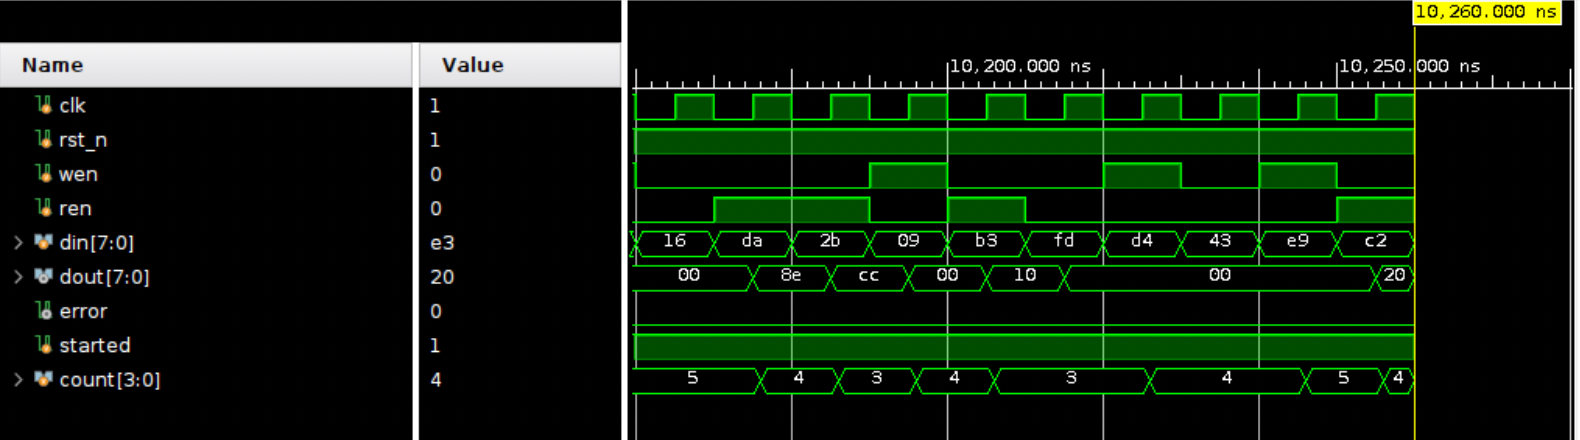
\includegraphics[width=0.9\textwidth]{./img/Q2-tb-wave1.png}
  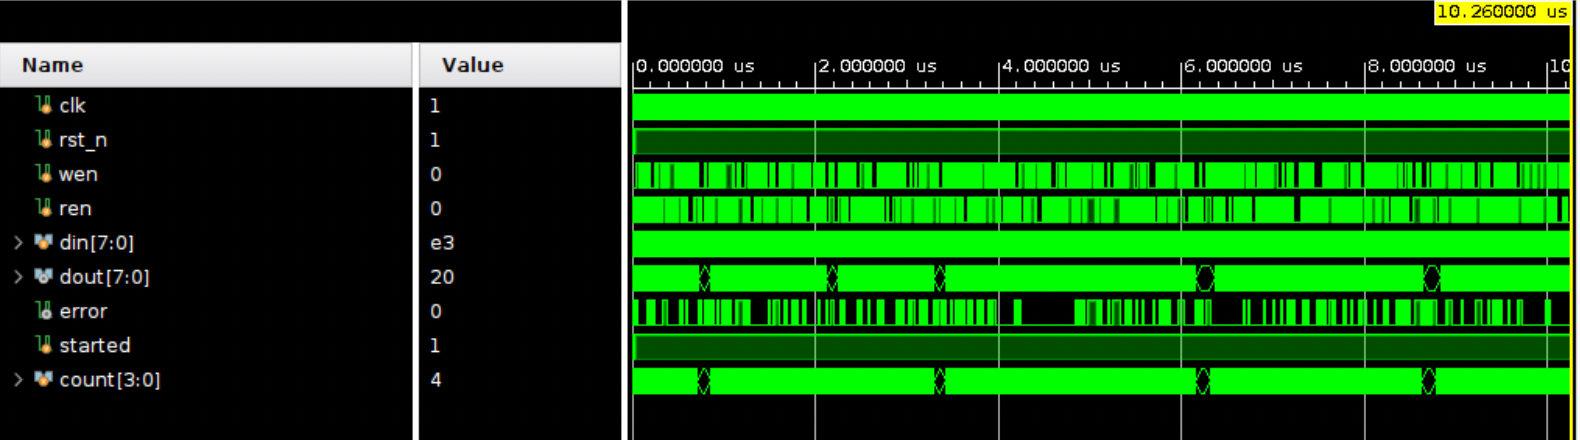
\includegraphics[width=0.9\textwidth]{./img/Q2-tb-wave2.png}
  \caption{Q2 Testbench Wave}
  \label{fig:Q2-tb}
\end{figure}

\newpage

\section{Q3: Multi-Bank Memory}
\label{sec:Q3}

\subsection{Implement}

這題需要實作一個 Multi-Bank Memory,每個 Bank 有 4 個 Sub-Bank,\
每個 Sub-Bank 由 128 個 8-bit memory 組成,總共有 4 個 Bank,如下圖 \ref{fig:Q3-spec} 所示。

\begin{figure}[!h]
  \centering
  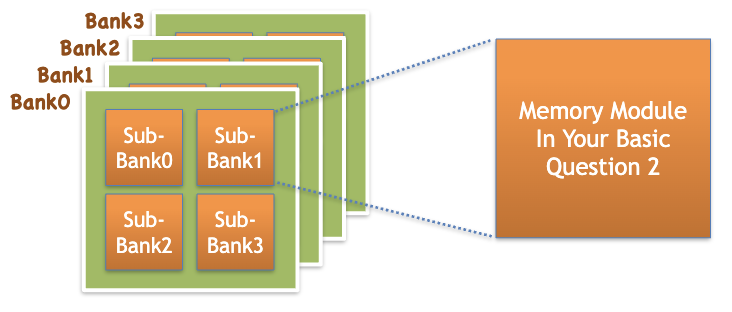
\includegraphics[width=0.9\textwidth]{./img/Q3-spec.png}
  \caption{Q3 Spec}
  \label{fig:Q2-spec}
\end{figure}

輸入的部分由以下幾個部分組成:
\begin{itemize}
  \item $ren, wen$:是否讀取或寫入
  \item $raddr$(11 bit):讀取的位址,前兩個 Bit 代表著是第幾個 Bank,接下來的兩個代表的是第幾個 Subbank。
  \item $waddr$ (11 bit):寫入的位址,格式同上
  \item $din$ (8 bit):寫入的資料
\end{itemize}



\subsubsection*{Bank}

\begin{itemize}
  \item input ren, wen:讀取或寫入的信號
  \item input [8:0] raddr, waddr:讀取或寫入的位址,前 2 Bit 代表是哪個記憶體單位,後 7 個則是該記憶體單位內的位址
  \item input [7:0] din:寫入的資料
  \item output [7:0] dout:讀取的資料(只在 ren = 1 時有意義)
\end{itemize}

這邊首先建立了四個長度 128,位寬 8-bit 的記憶體,而我們要做的事就是正確的算出要輸入到記憶體的參數是什麼:
\begin{itemize}
  \item $ren$:利用與 $raddr[8:7] == i\ (i \in [0, 3])$ 做 AND 運算,來決定這個記憶體單位要不要讀取
  \item $wen$:與 $ren$ 的處理方式一樣,只是改成使用 $waddr$ 來判斷。
  \item $address$:透過三元運算子,當 $ren = 1$ 時,將 $address$ 設為 $raddr$,否則就設為 $waddr$
\end{itemize}


\subsubsection*{主 Module}

主要的 Module 負責整體的輸入輸出,將輸入的參數正確的分配給各個 Bank,\
並將正確的 Bank 輸出導向至最後的輸出。

在處理輸入的部分,主要分為以下步驟:
\begin{itemize}
  \item $ren$:直接利用 $ren \& (raddr[10:9]) == i\ (i \in [0, 3])$ 的方式來決定每個 Bank 的 $ren$
  \item $wen$:分為兩個步驟
  \begin{enumerate}
    \item 判斷是否能夠輸入,題目規定,當要求同時讀寫同一個 Sub-bank 時,就以讀的操作為主,因此先利用\
    \texttt{wen \&\& (ren == 0 || (waddr[10:7] != raddr[10:7]))} 判斷出這次的寫入操作是否合法
    \item 與 $ren$ 用一樣的方式將上述的信號分配到正確的 Bank
  \end{enumerate}
\end{itemize}

至於輸出的部分,我使用了四個 8 bit 的 wire: $out[3:0]$,分別接至四個 Bank 的輸出,\
由於在處理輸入信號的部分,當該 Bank 不是要求的 Bank 時,output 會直接是 $0$,\
因此要取得正確的輸出就只要將四個 output 做 Bitwise OR 即可。

\newpage

\subsection{Circuit}

\subsubsection*{Memory}
這部分沿用的是前面提到的 Memory,將其長度擴充為 128,由於篇幅關係就不額外展示長度 128 的電路圖。

\subsubsection*{Bank}



首先,利用 Mux,以 ren 作為 sel bit,判斷出要操作的 address 是哪一個。\
若 $ren = true$,就選擇 raddr 的後七個 bit,否則就選擇 waddr 的後七個 bit。
\par
接著使用比較器,用 $waddr, raddr$ 的前兩個 bit 與 $0 \sim 3$ 做比較,\
找出實際要發出訊號的記憶體單位是哪一個,最後再分別跟 $ren, wen$ 做 AND 運算,\
確保是做哪個操作後,就能夠將訊號傳遞至記憶體單位。
\par
由於只會有一個記憶體單位有輸出值(其他都會被設定為 0),因此最後直接將 4 個記憶體單位的輸出做 Bitwise OR 就能夠得到最後的輸出。\
如圖 \ref{fig:Q3-Bank} 所示。


\begin{figure}[!h]
  \centering
  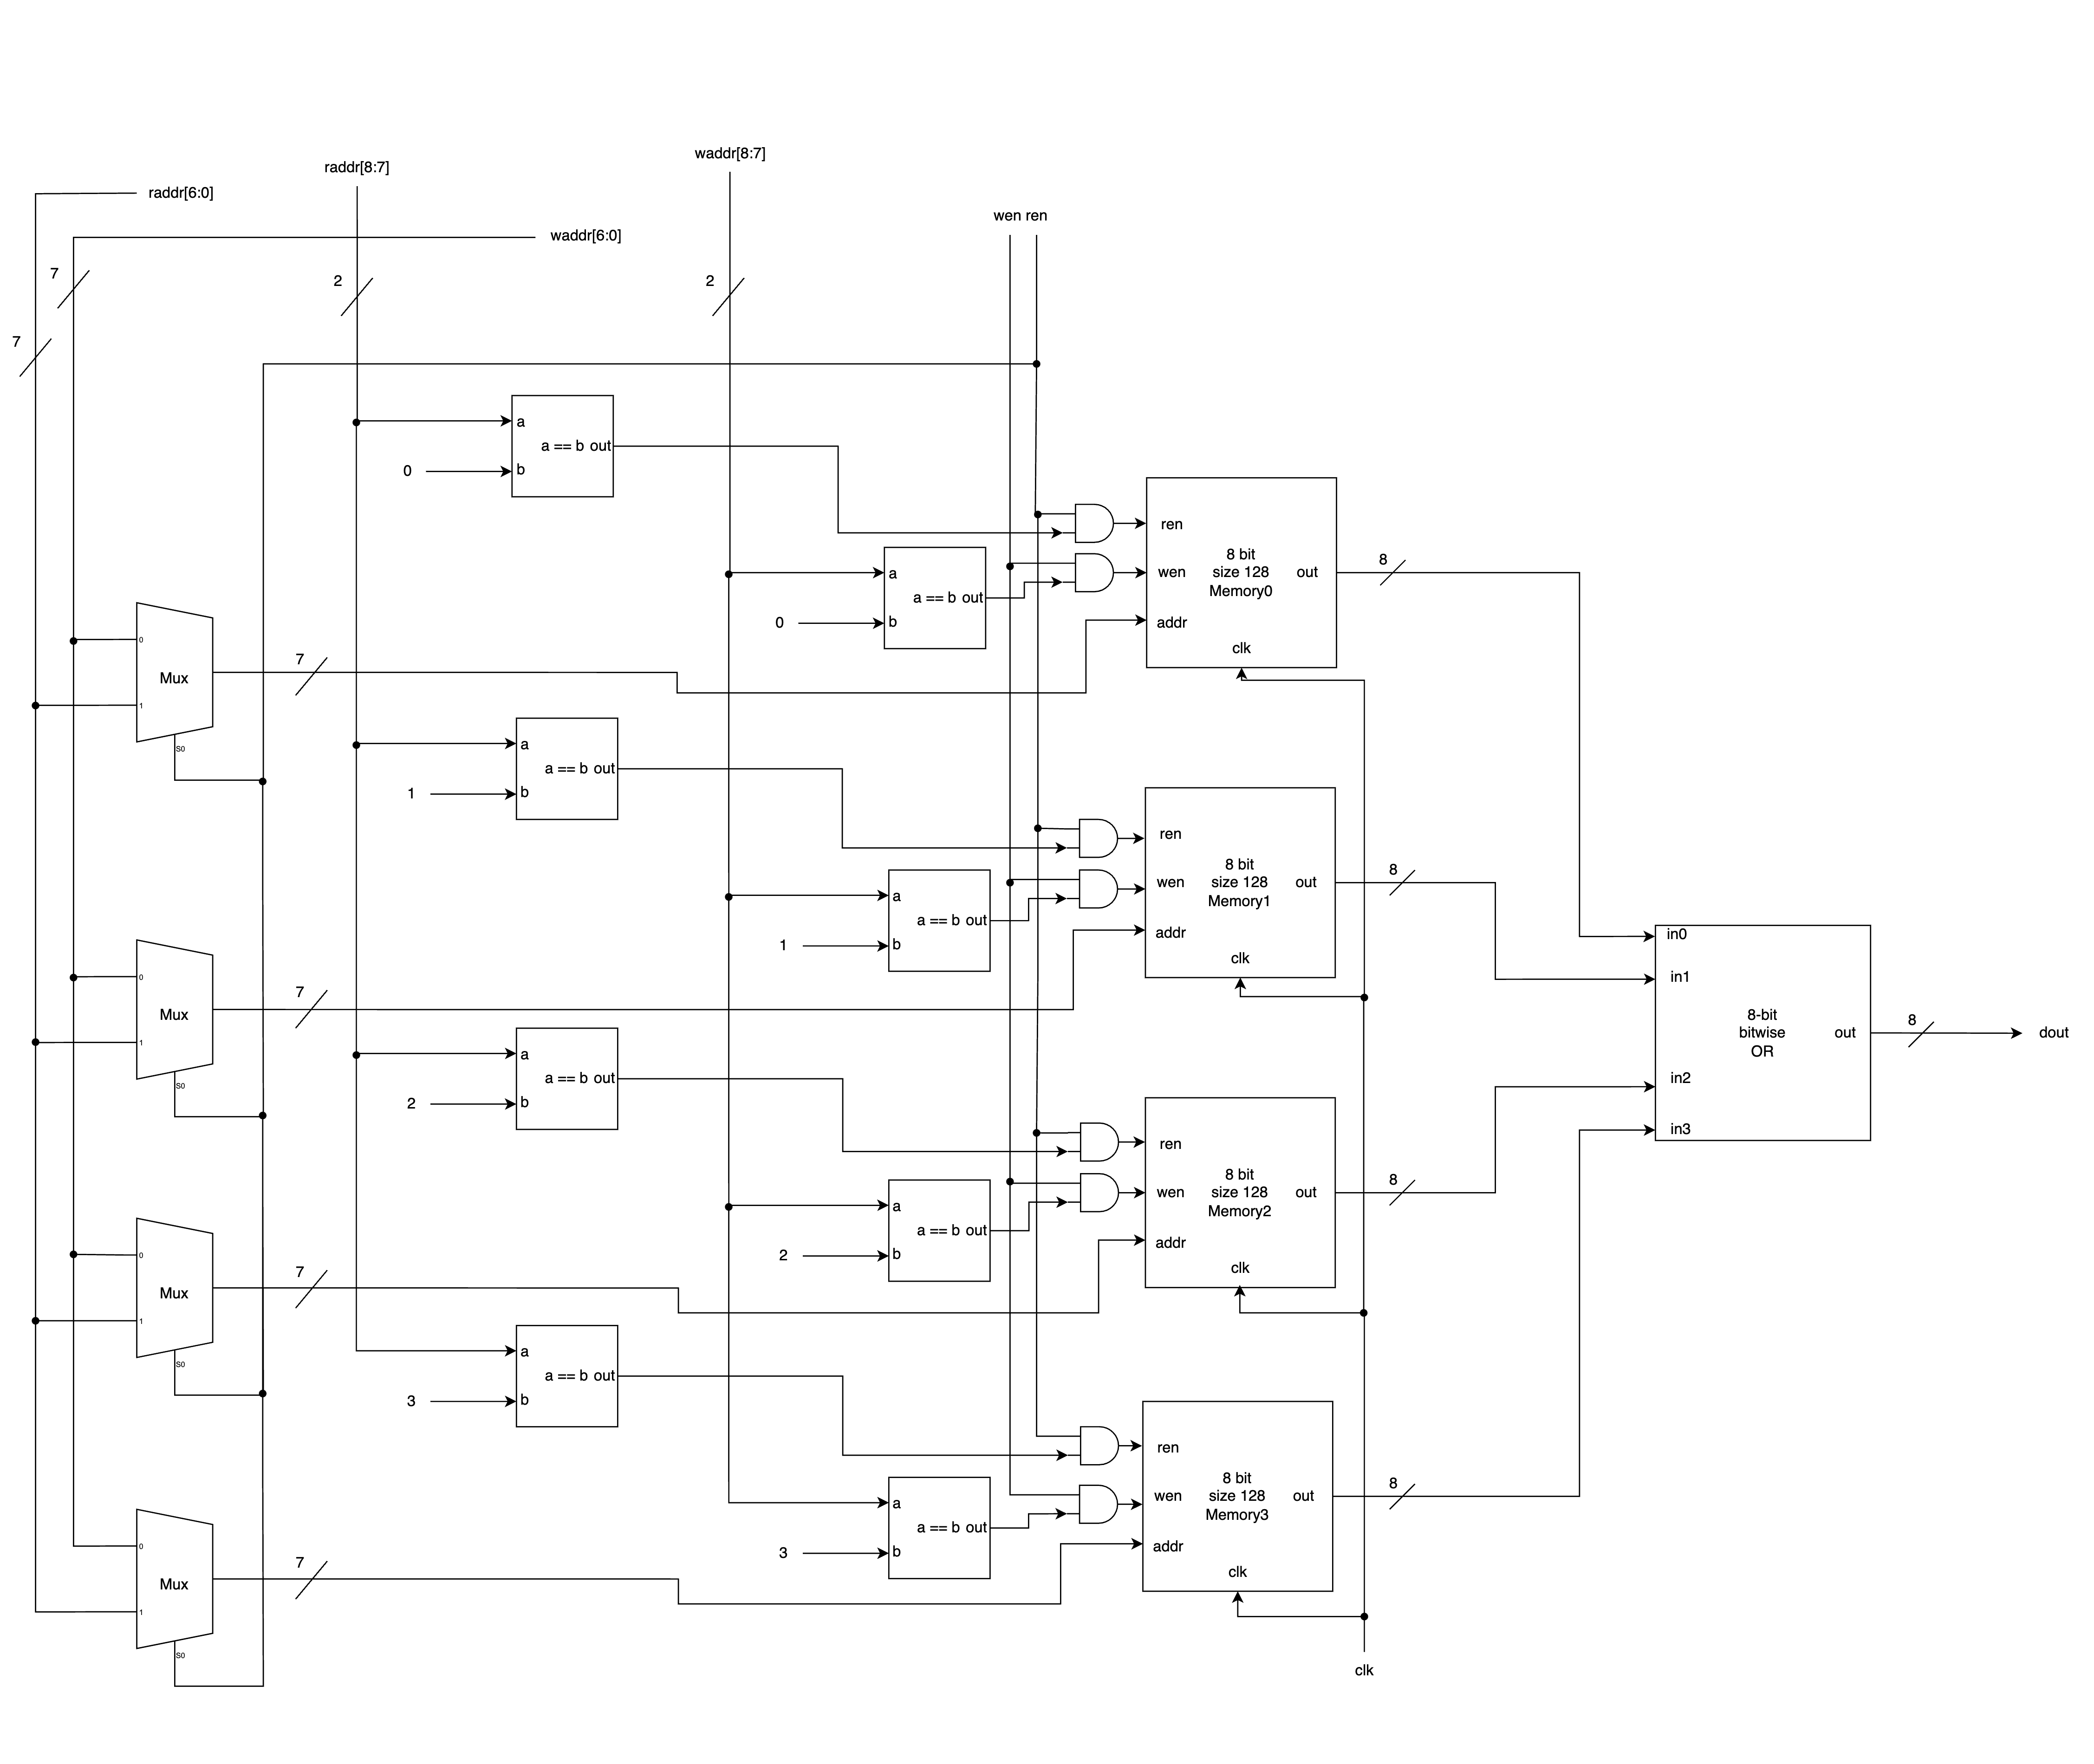
\includegraphics[width=\textwidth]{./img/Q3-Bank.png}
  \caption{Q3 Bank}
  \label{fig:Q3-Bank}
\end{figure}
\newpage

\subsubsection*{Main Module}
與 Bank 的實作方法類似,不過因為同一個記憶體區塊不能同時讀寫的緣故,因此 $wen$ 使用了\
不等於的比較器,比較 $waddr, raddr$ 的前四個 bit 是否不同,若是不同則將 $wen$ 設為 $0$\
如圖 \ref{fig:Q3-main} 所示。


\begin{figure}[!h]
  \centering
  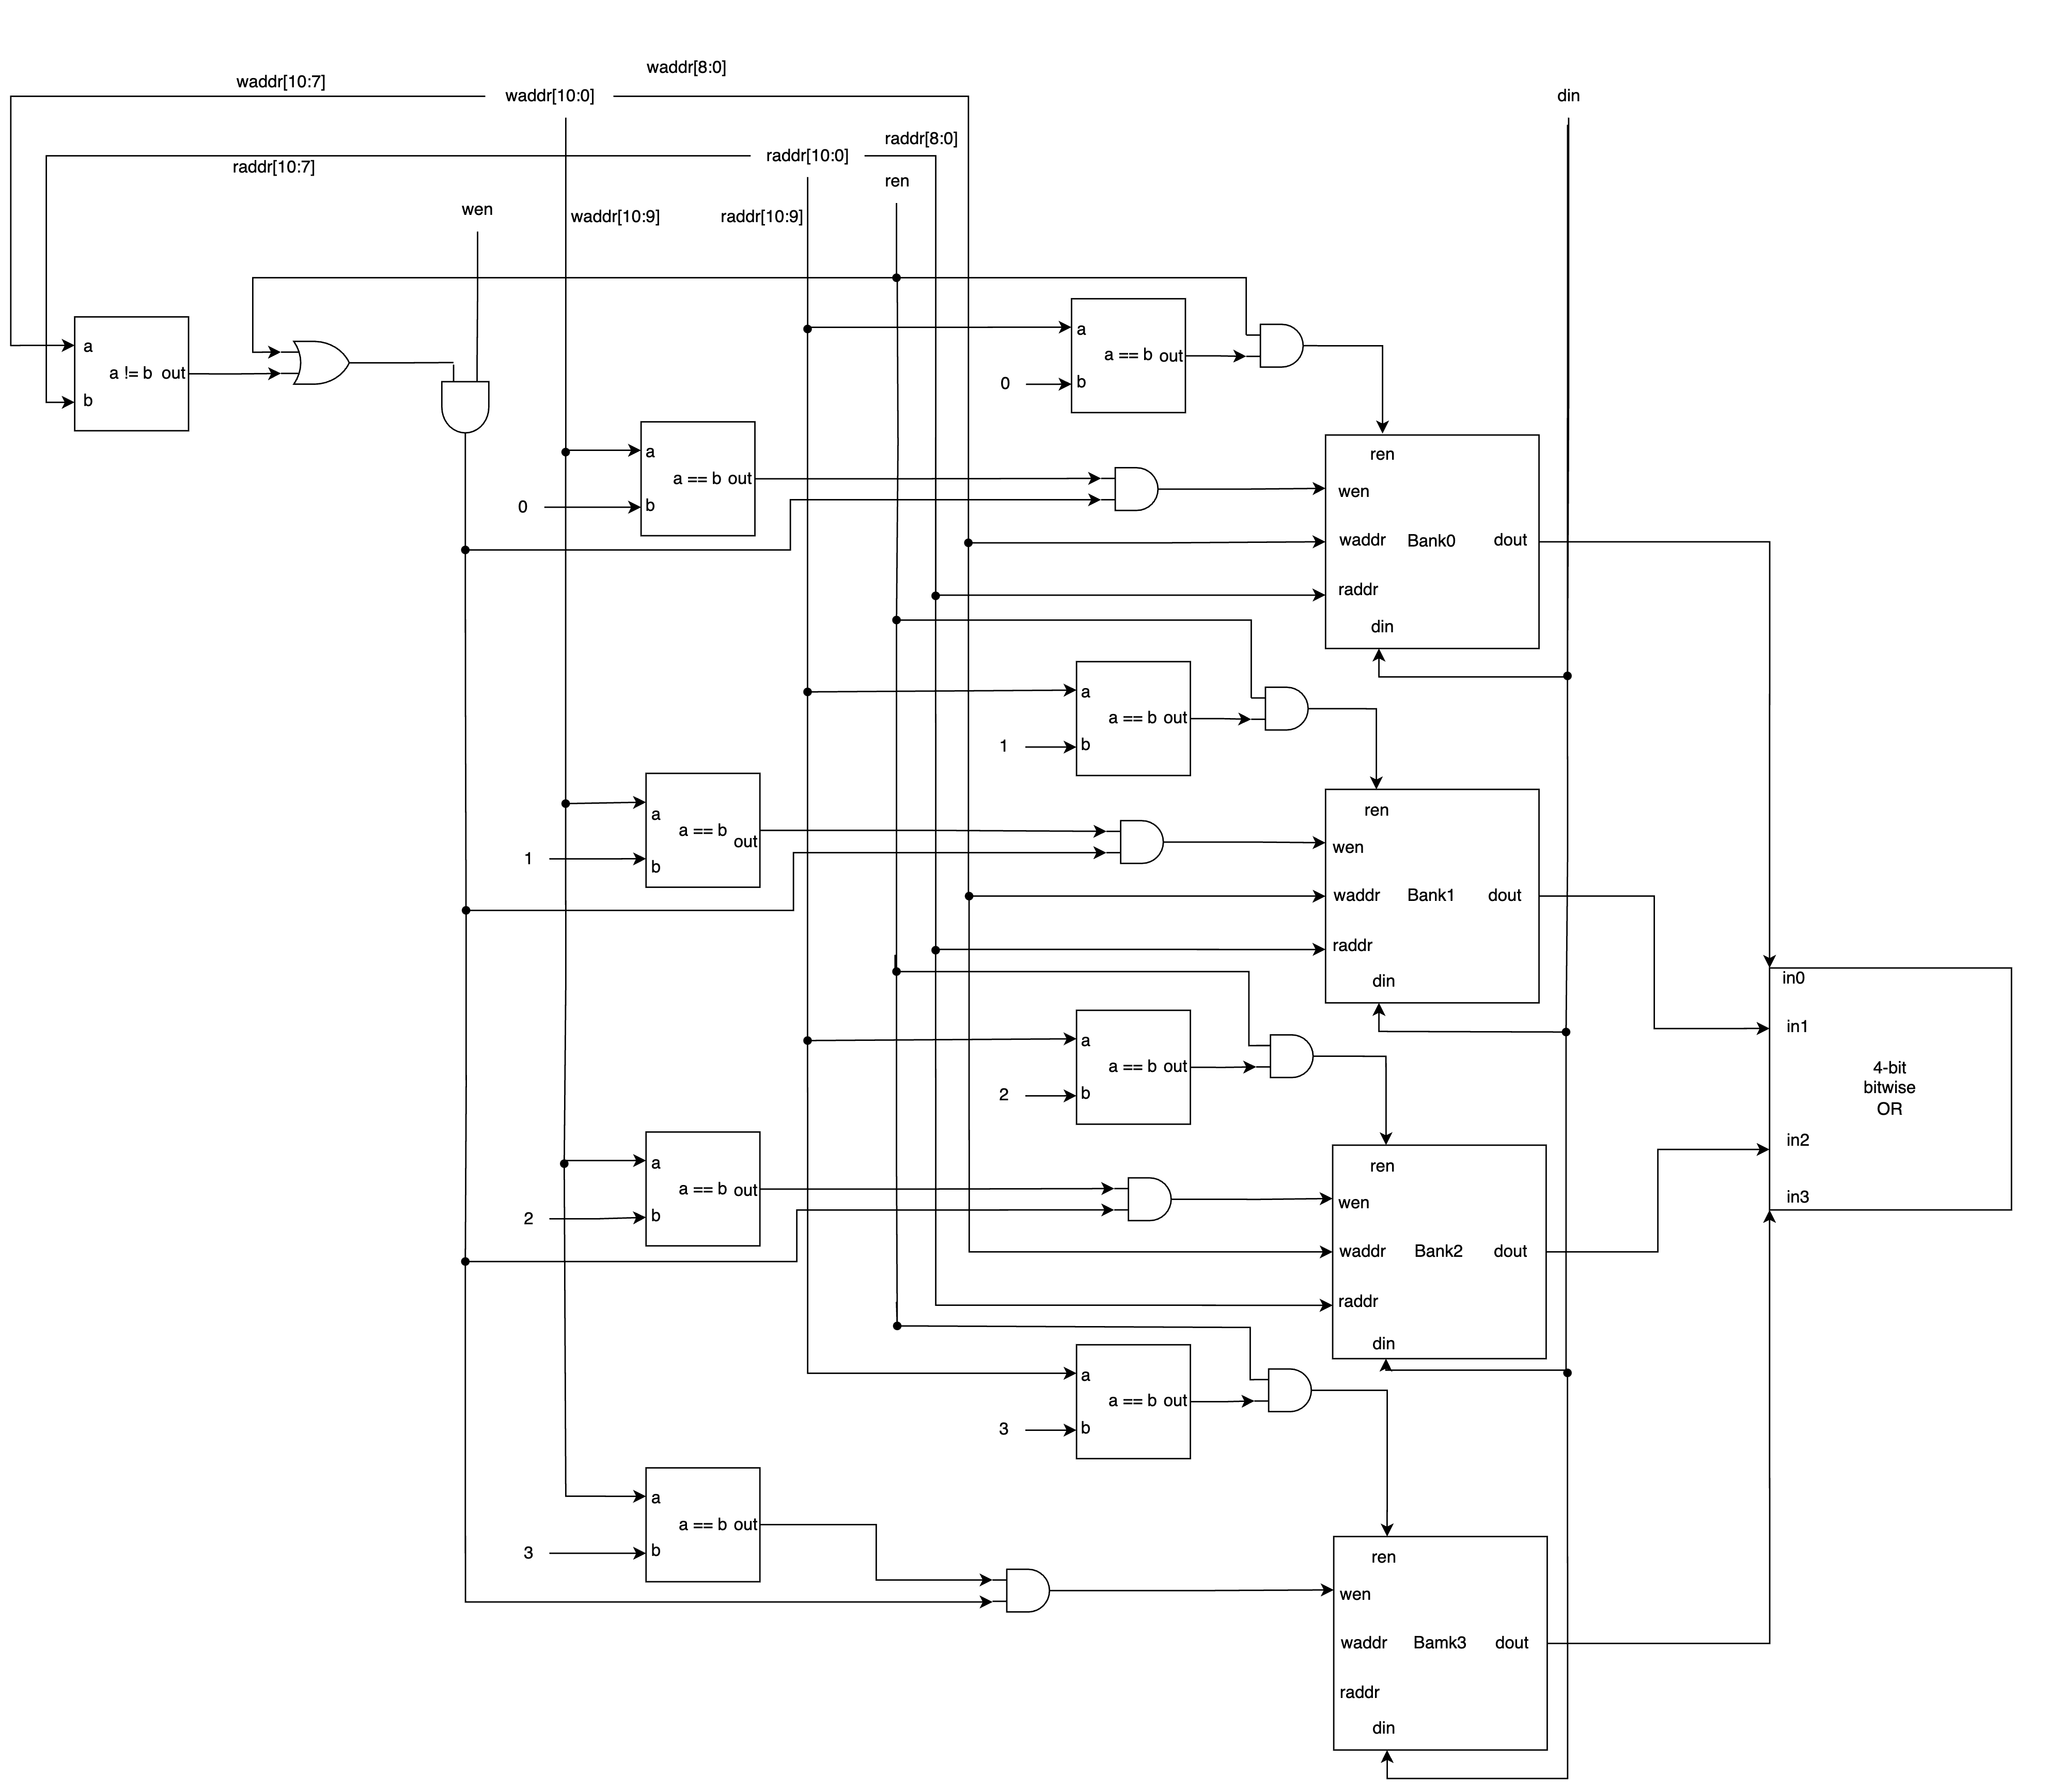
\includegraphics[width=\textwidth]{./img/Q3.png}
  \caption{Q3 Main Module}
  \label{fig:Q3-main}
\end{figure}

\newpage


\section{Q4: Round-Robin FIFO Arbiter}
\begin{itemize}
  \item input clk: clock
  \item input rst\_n: 重置信號
  \item input [3:0] wen:四個 bit 的寫入信號,$wen[i]$ 代表第 $i$ 個 Queue 是否要輸入
  \item input [7:0] a, b, c, d:分別對應到 $i = 0, 1, 2, 3$ 的寫入資料
  \item output [7:0] dout:輸出的資料
  \item output valid:目前是否能夠輸出資料
\end{itemize}

這題需要實作一個 Arbiter,會根據 $wen$ 的訊號寫入 Queue 中,\
並輪流輸出 Queue 中的資料,大致上會有幾種情況:
\begin{itemize}
  \item 要輸出第 $i$ 個 Queue 的資料,但是該 Queue 正在被寫入:不輸出
  \item 要輸出第 $i$ 個 Queue 的資料,但是該 Queue 是空的:不輸出
  \item 要輸出第 $i$ 個 Queue 的資料,且該 Queue 有資料:輸出並 pop 該資料
\end{itemize}

\subsection{Implement}
首先使用四個章節 \ref{sec:Q2} 實作的 Queue,作為這題的儲存單位。
\par
接著是處理輸入的部分,由於這題是輸入優先,所以我們直接將 $wen[i]$ 以及 $a, b, c, d$作為\

四個 Queue 的 $wen$ 輸入,並將輸出導出到 $out[0] \sim out[3]$\
而 $ren$ 因為輸入優先,因此需要先與 $wen[i]$ 的反相做 AND 運算,\
才能夠保證輸出只有在沒有輸入的時候才會進行。
\par
接著是將 Queue 的輸出導向至 $dout$ 的部分,我使用一個 2-bit 的counter register,\
會在每個 posedge $+1$ 來創造 $0 \sim 3$ 的循環,並用來記錄目前是準備要讀第幾個 Queue,\
在第 $t$ 個 clock cycle 時,會透過當下 $counter$對應的 $ren[i]$ 向 Queue 發送讀取請求,\
而輸出會在下一個 clock cycle: $t + 1$ 被更新到對應的 $out[i]$。
\par
不過輸出會有兩種情況:合法與不合法:
\begin{itemize}
  \item 不合法:當 Queue 無法執行該操作時,會透過 $error[i]$ 輸出 error 訊號\
  ,並在 $t + 1$ 時被更新,再與對應的 $wen[i]$ 做 OR 並反相就是 valid 的數值。\
  不過因為 $wen[i]$ 並不像 $error[i]$ 一樣,會在 clock posedge 更新,\
  因此先將 $wen[i]$ 儲存在一個 register 中,將數值調整為與 clock 同步後,再與 $error[i] 做反向即可$。
  \item 合法:將對應的 $out[i]$ 導向至 dout,但由於收到 FIFO 的值是在 $t + 1$ 的時候,\
  因此此時需要輸出的答案是 $out[counter - 1]$ 的值,\
  
\end{itemize}

\newpage
\subsection{Circuit}
首先介紹一個 4-bit 的 Shifter,能夠指定將輸入的數字往左位移 $shift$ 次,由四個 4-bit 4-to-1 MUX 組成。

\begin{figure}[!h]
  \centering
  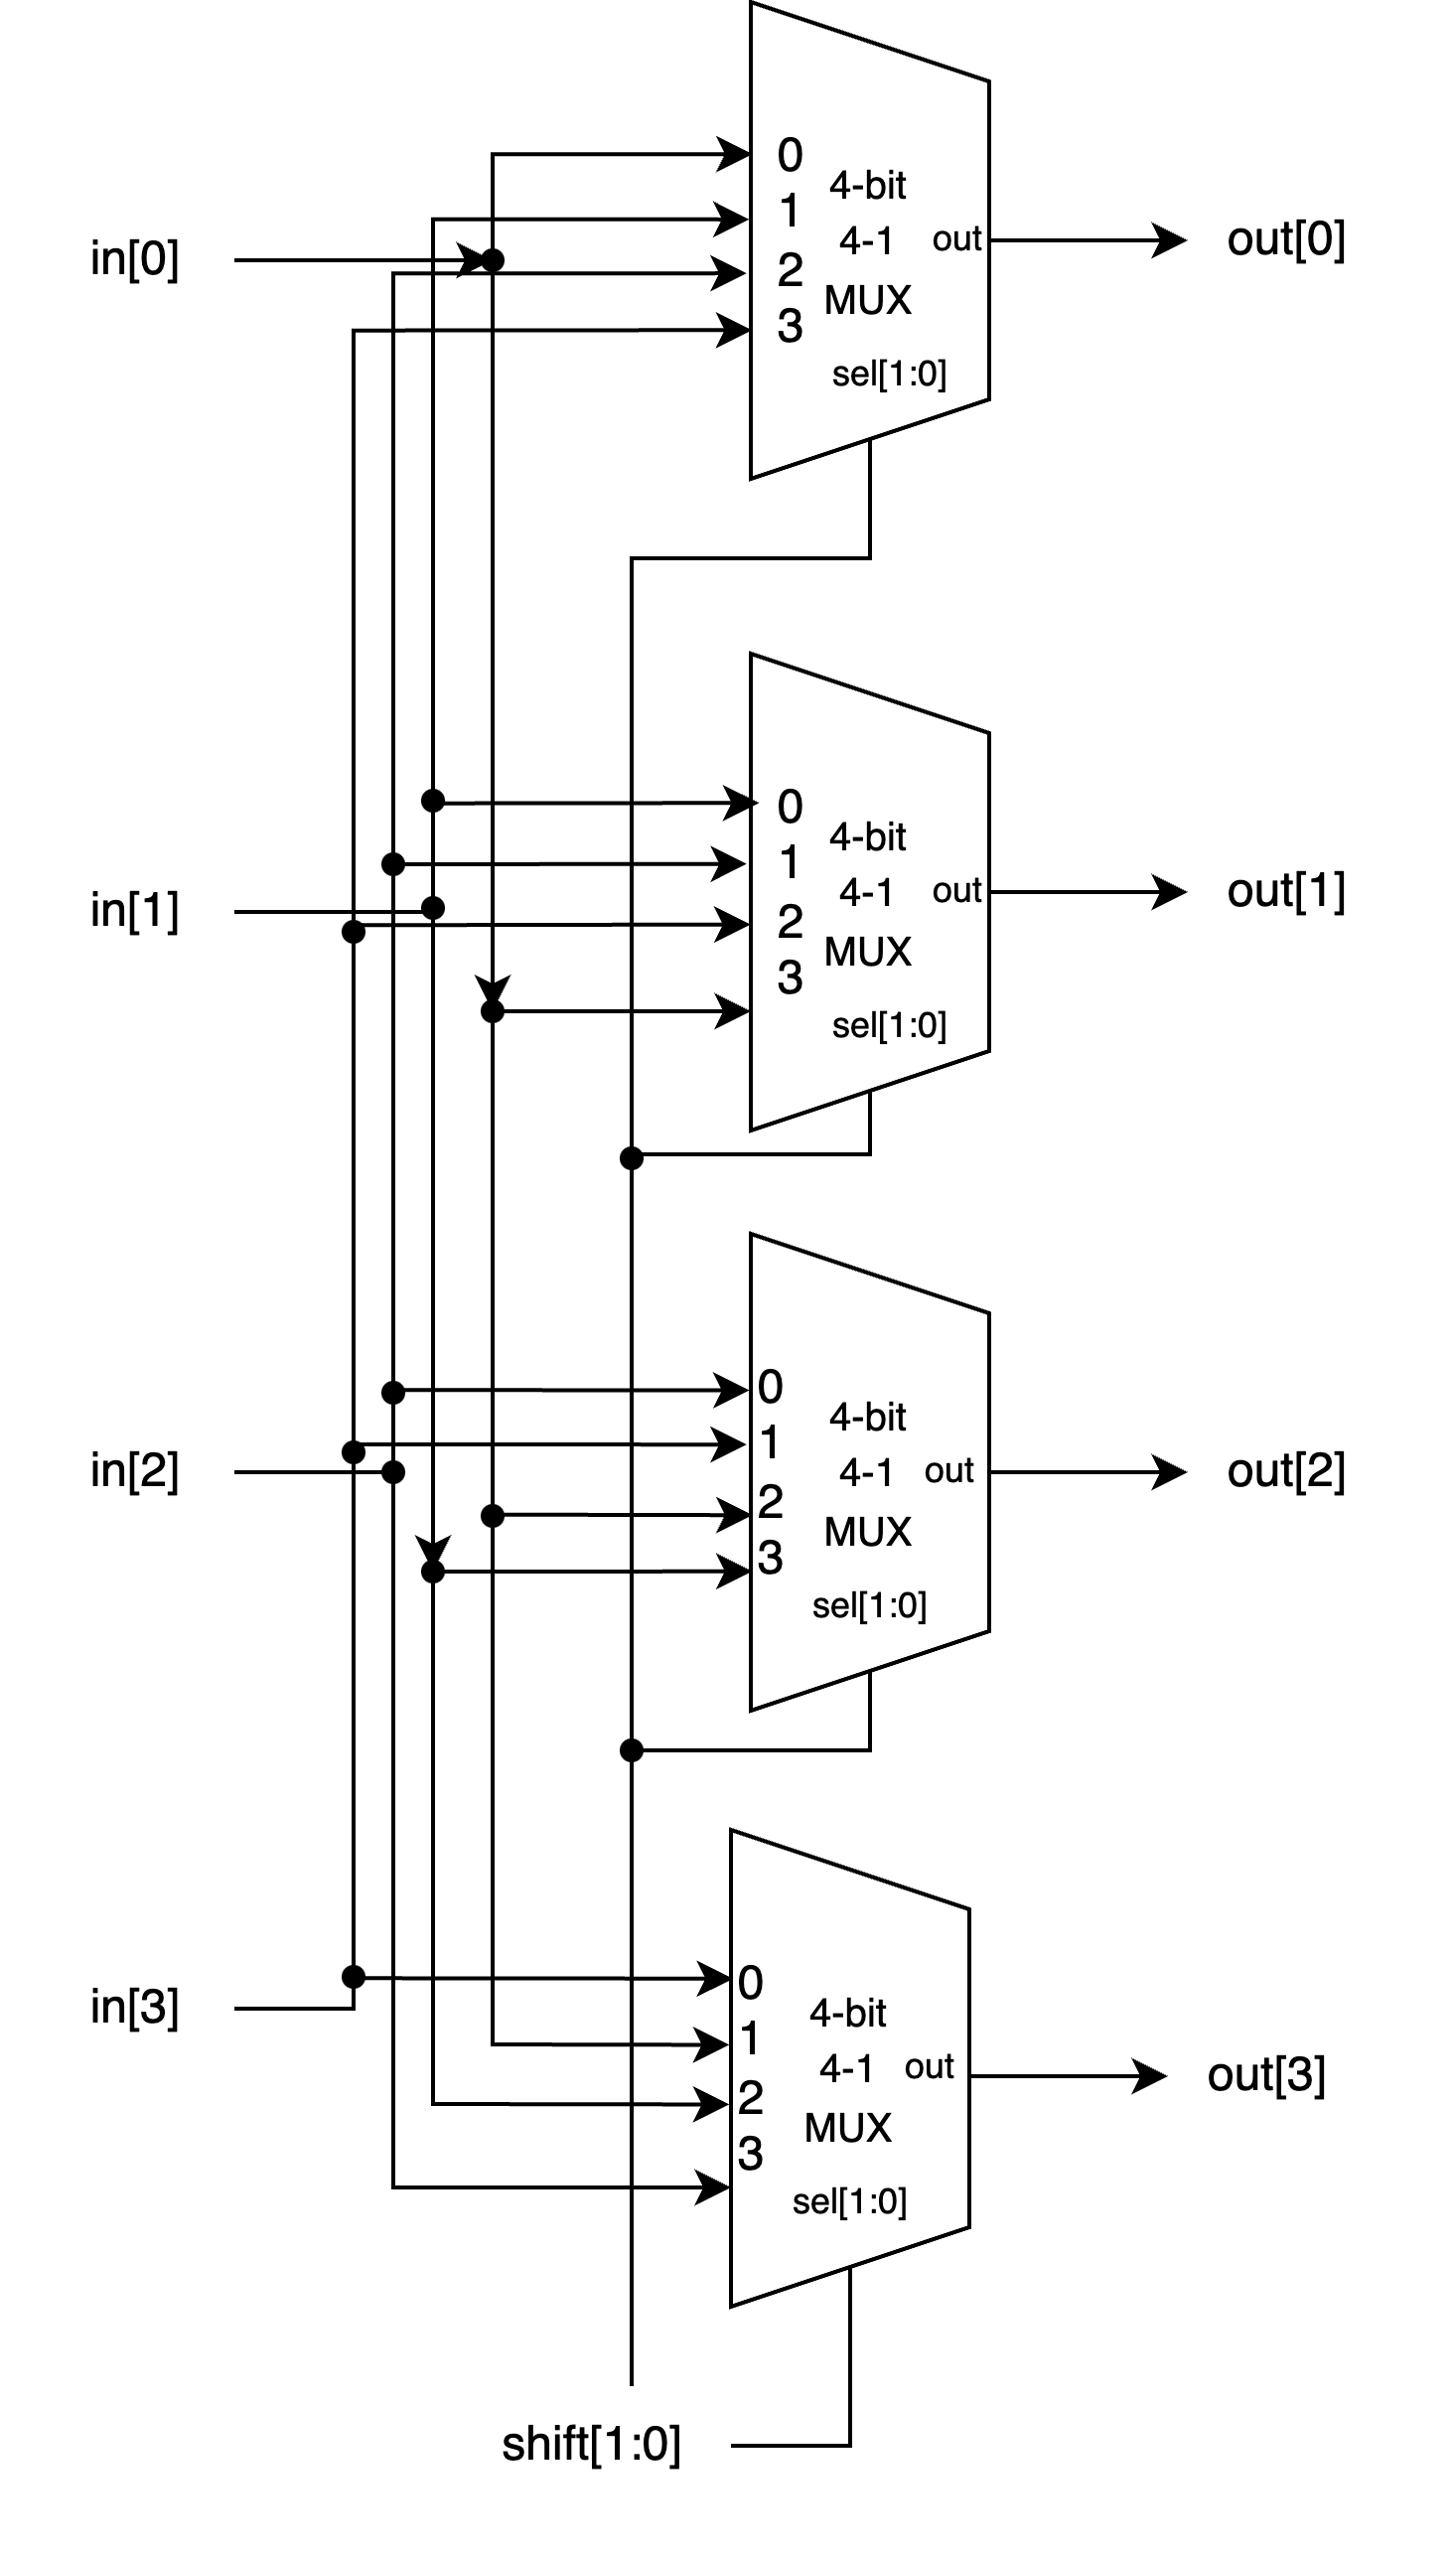
\includegraphics[width=0.6\textwidth]{./img/Q4-Shift.png}
  \caption{Q4 Shifter}
  \label{fig:Q4-shift}
\end{figure}

\newpage

接著是整體的電路實作,基本上分為三層:
\subsubsection*{輸入層}
\begin{itemize}
  \item ren:透過 left shift $0001$ $i$ 次的方式,來指定 $ren$ 的第幾個位元要是 true
  \item counter:每個 clock cycle 會加一,由於是 2-bit 的關係,因此數到 $4$ 時會自動歸零為 $0$
  \item wenc:將 $wen$ 存進去,使其與 clock 同步
\end{itemize}

\subsubsection*{計算層}
將輸入的 $wen$ 以及計算出來的 $ren$ 傳到 Queue 中

\subsubsection*{輸出層}
透過以 $counter$ 作為 sel bit 的 MUX 判斷要輸出哪一個 output 的值,\
但由於當 $error$ 發生的時候有可能得到 X 的輸出,因此在最後再加一個 2-to-1 MUX,\
用 $valid$ 當作 sel bit,在發生不合法的情況時直接輸出 $0$。

\begin{figure}[!h]
  \centering
  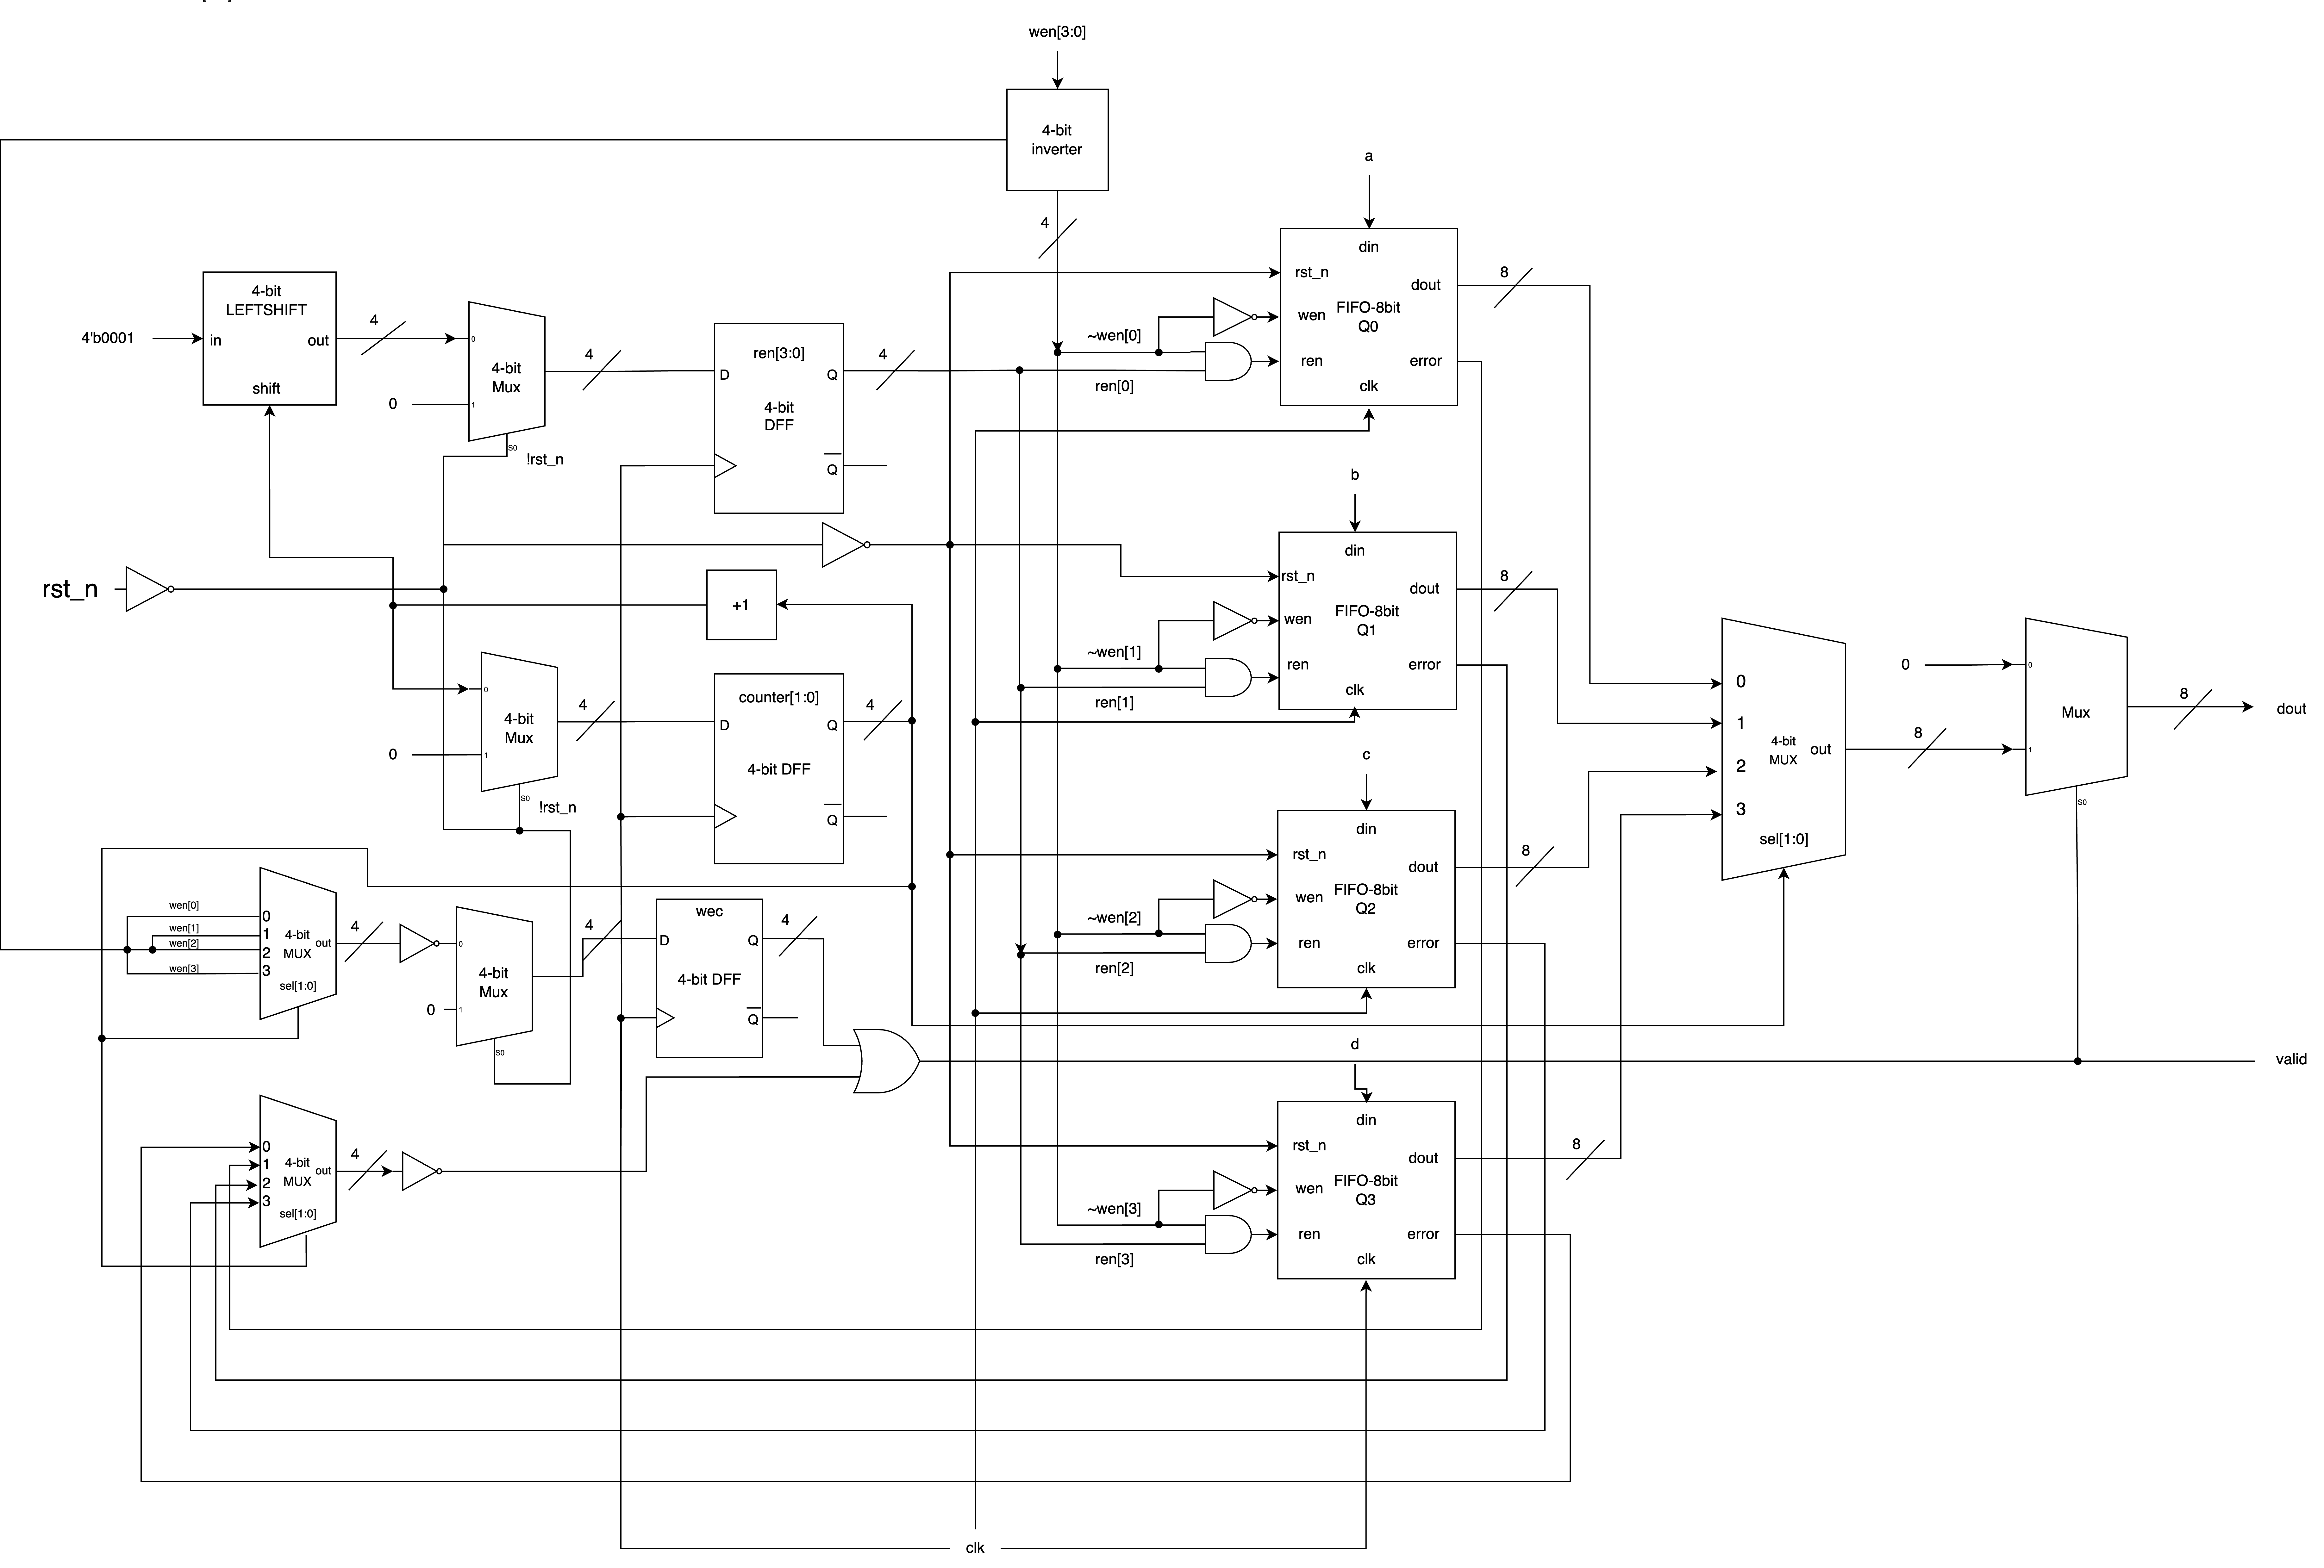
\includegraphics[width=\textwidth]{./img/Q4.png}
  \caption{Q4 Circuit}
  \label{fig:Q4}
\end{figure}

\newpage

\subsection{Testbench}

首先重現了題目範例中的波形圖:

\begin{figure}[!h]
  \centering
  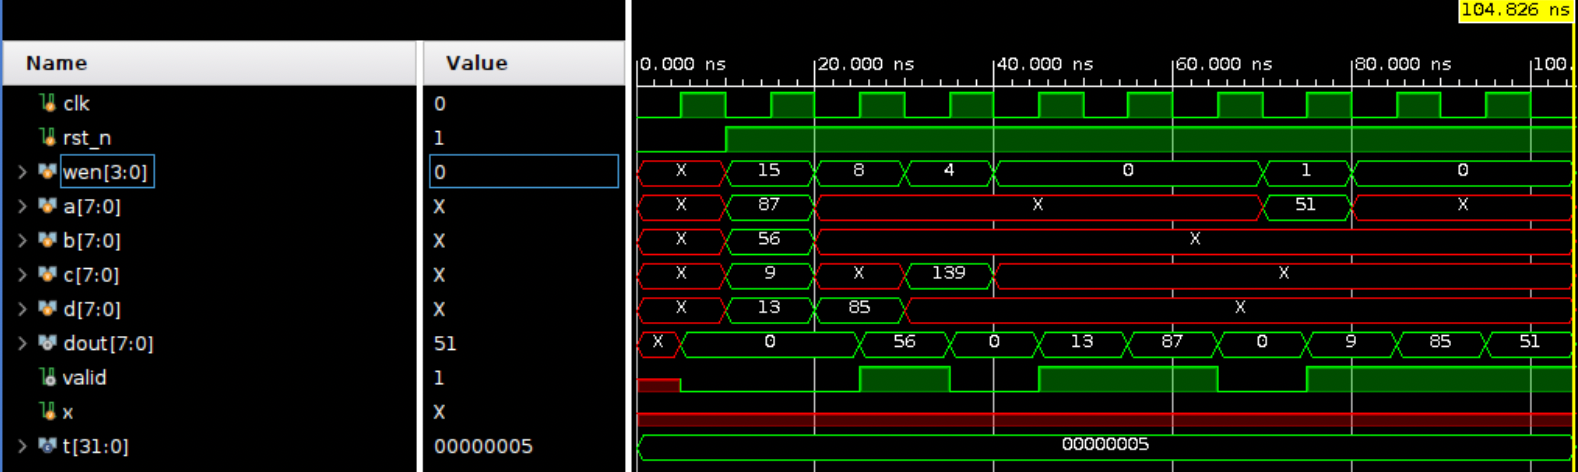
\includegraphics[width=\textwidth]{./img/Q4-tb-ex.png}
  \caption{Q4 Example Testbench}
  \label{fig:Q4-tb-ex}
\end{figure}

接著再使用 random 來進行額外的模擬,並觀察是否與期望相符。

\begin{figure}[!h]
  \centering
  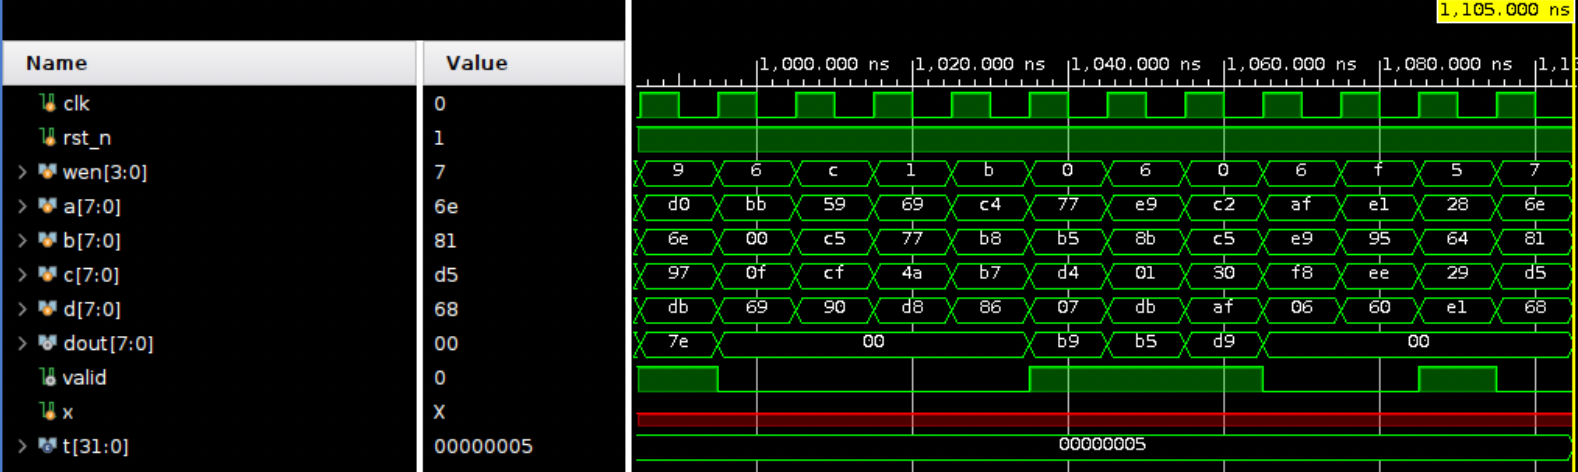
\includegraphics[width=\textwidth]{./img/Q4-tb-wave1.png}
  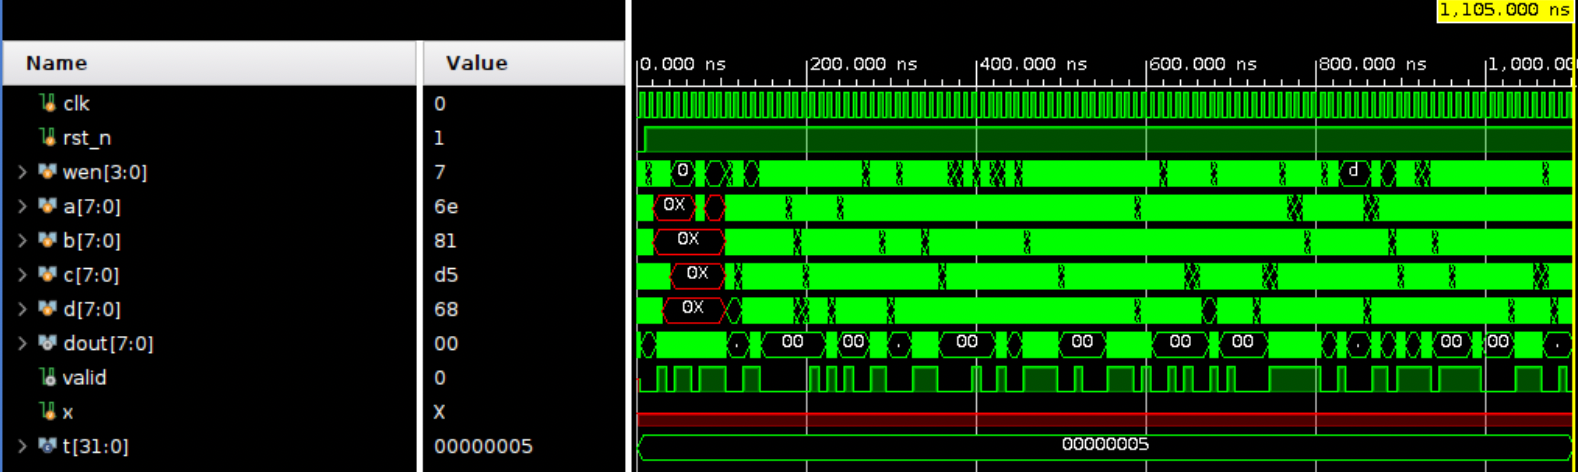
\includegraphics[width=\textwidth]{./img/Q4-tb-wave2.png}
  \caption{Q4 Testbench Wave}
  \label{fig:Q4-tb}
\end{figure}

\newpage

\section{Q5: 4-bit Parameterized Ping-Pong Counter}

\subsection{Implement}

\begin{itemize}
  \item input clk: clock
  \item input rst\_n:重置信號
  \item input flip:是否翻轉
  \item input [3:0] max:最大值
  \item input [3:0] min:最小值
  \item output direction:Counter 變化方向
  \item output [3:0] out:輸出的值
\end{itemize}

這題與 Q1 類似,不過加入了 $min, max, flip$ 的參數,\
代表 Counter 能夠達到的最大值、最小值,以及是否要翻轉方向。

\subsection{Circuit}

output 的計算會經過幾個步驟:
\begin{enumerate}
  \item 判斷 $out$ 是否已經達到邊界,若是碰到上界,將 $direction$ 設為 $0$、$out - 1$,\
  反之則設為 $1$、$out + 1$
  \item 判斷是否已經開始($start = 1$)、是否啟用($enable = 1$)、是否符合範圍($out \in [min, max]$),\
  若是的話,則:
  \begin{itemize}
    \item $out = max$:將 $direction$ 設為 $0$、$out - 1$
    \item $out = min$:將 $direction$ 設為 $1$、$out + 1$
    \item 其他情況:根據 $direction$ 進行加減
  \end{itemize}
  否則就讓 $direction$ 保持原樣
  \item 判斷是否需要翻轉,是的話則反轉 direction,並依據 direction 進行加減
  \item 判斷是否啟用,是的話套用以上的結果,否則話則保持原樣
  \item 判斷是否需要 reset,是的話將 $direction$ 設為 $1$、$out$ 設為 $0$,否則保持以上結果
\end{enumerate}

\newpage

\begin{figure}[!h]
  \centering
  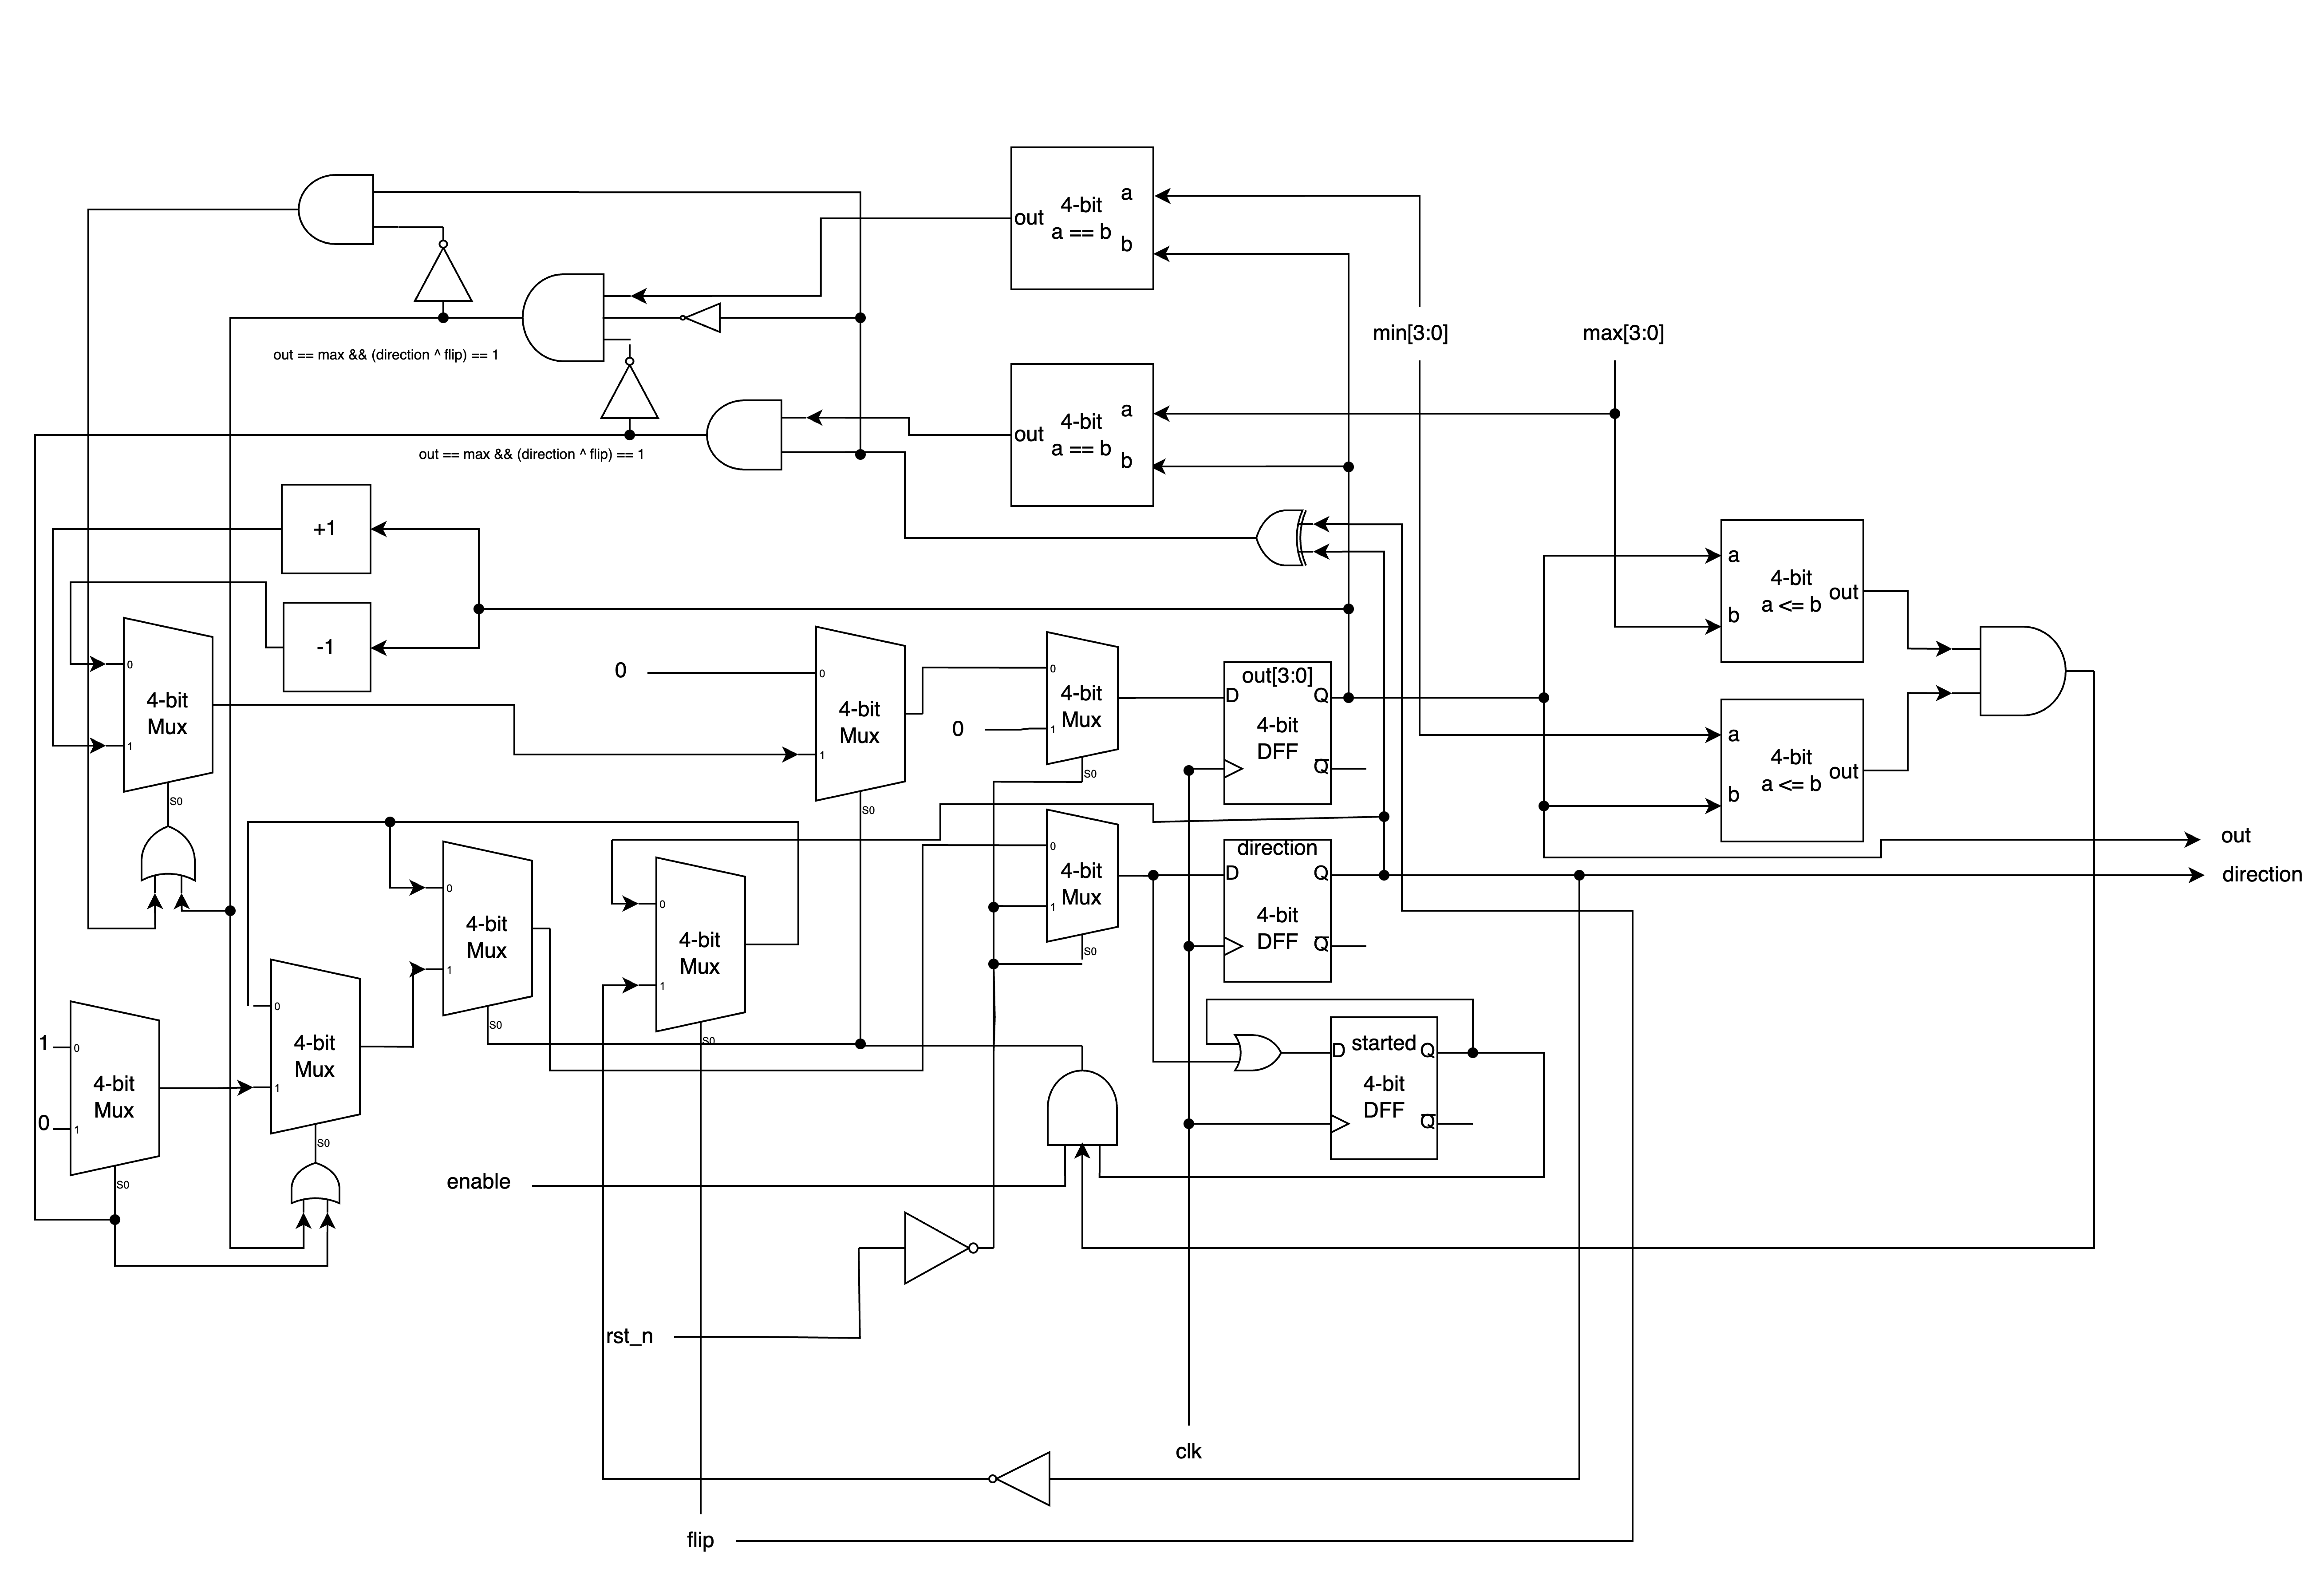
\includegraphics[width=\textwidth]{./img/Q5.png}
  \caption{Q5 Circuit}
  \label{fig:Q5}
\end{figure}


\newpage

\section{FPGA: 4-bit Paramterized Ping-Pong Counter on FPGA}

這題需要將上個問題的 Counter 實作在 FPGA 上,並透過以下接口作為輸入輸出:
\begin{itemize}
  \item $SW[15]$: enable
  \item $SW[14:11]$: max
  \item $SW[10:7]$: min
  \item Button Down: flip
  \item Button UP: reset
  \item 7-segment-display: out
\end{itemize}


我們寫了一個 Display Control 模組,用來運算 Counter 的輸入以及七段顯示器的輸出,而 Counter 則是沿用上一題的實作稍作修改,加上了 $cnt\_en$ 這個訊號。

\begin{figure}[!h]
  \centering
  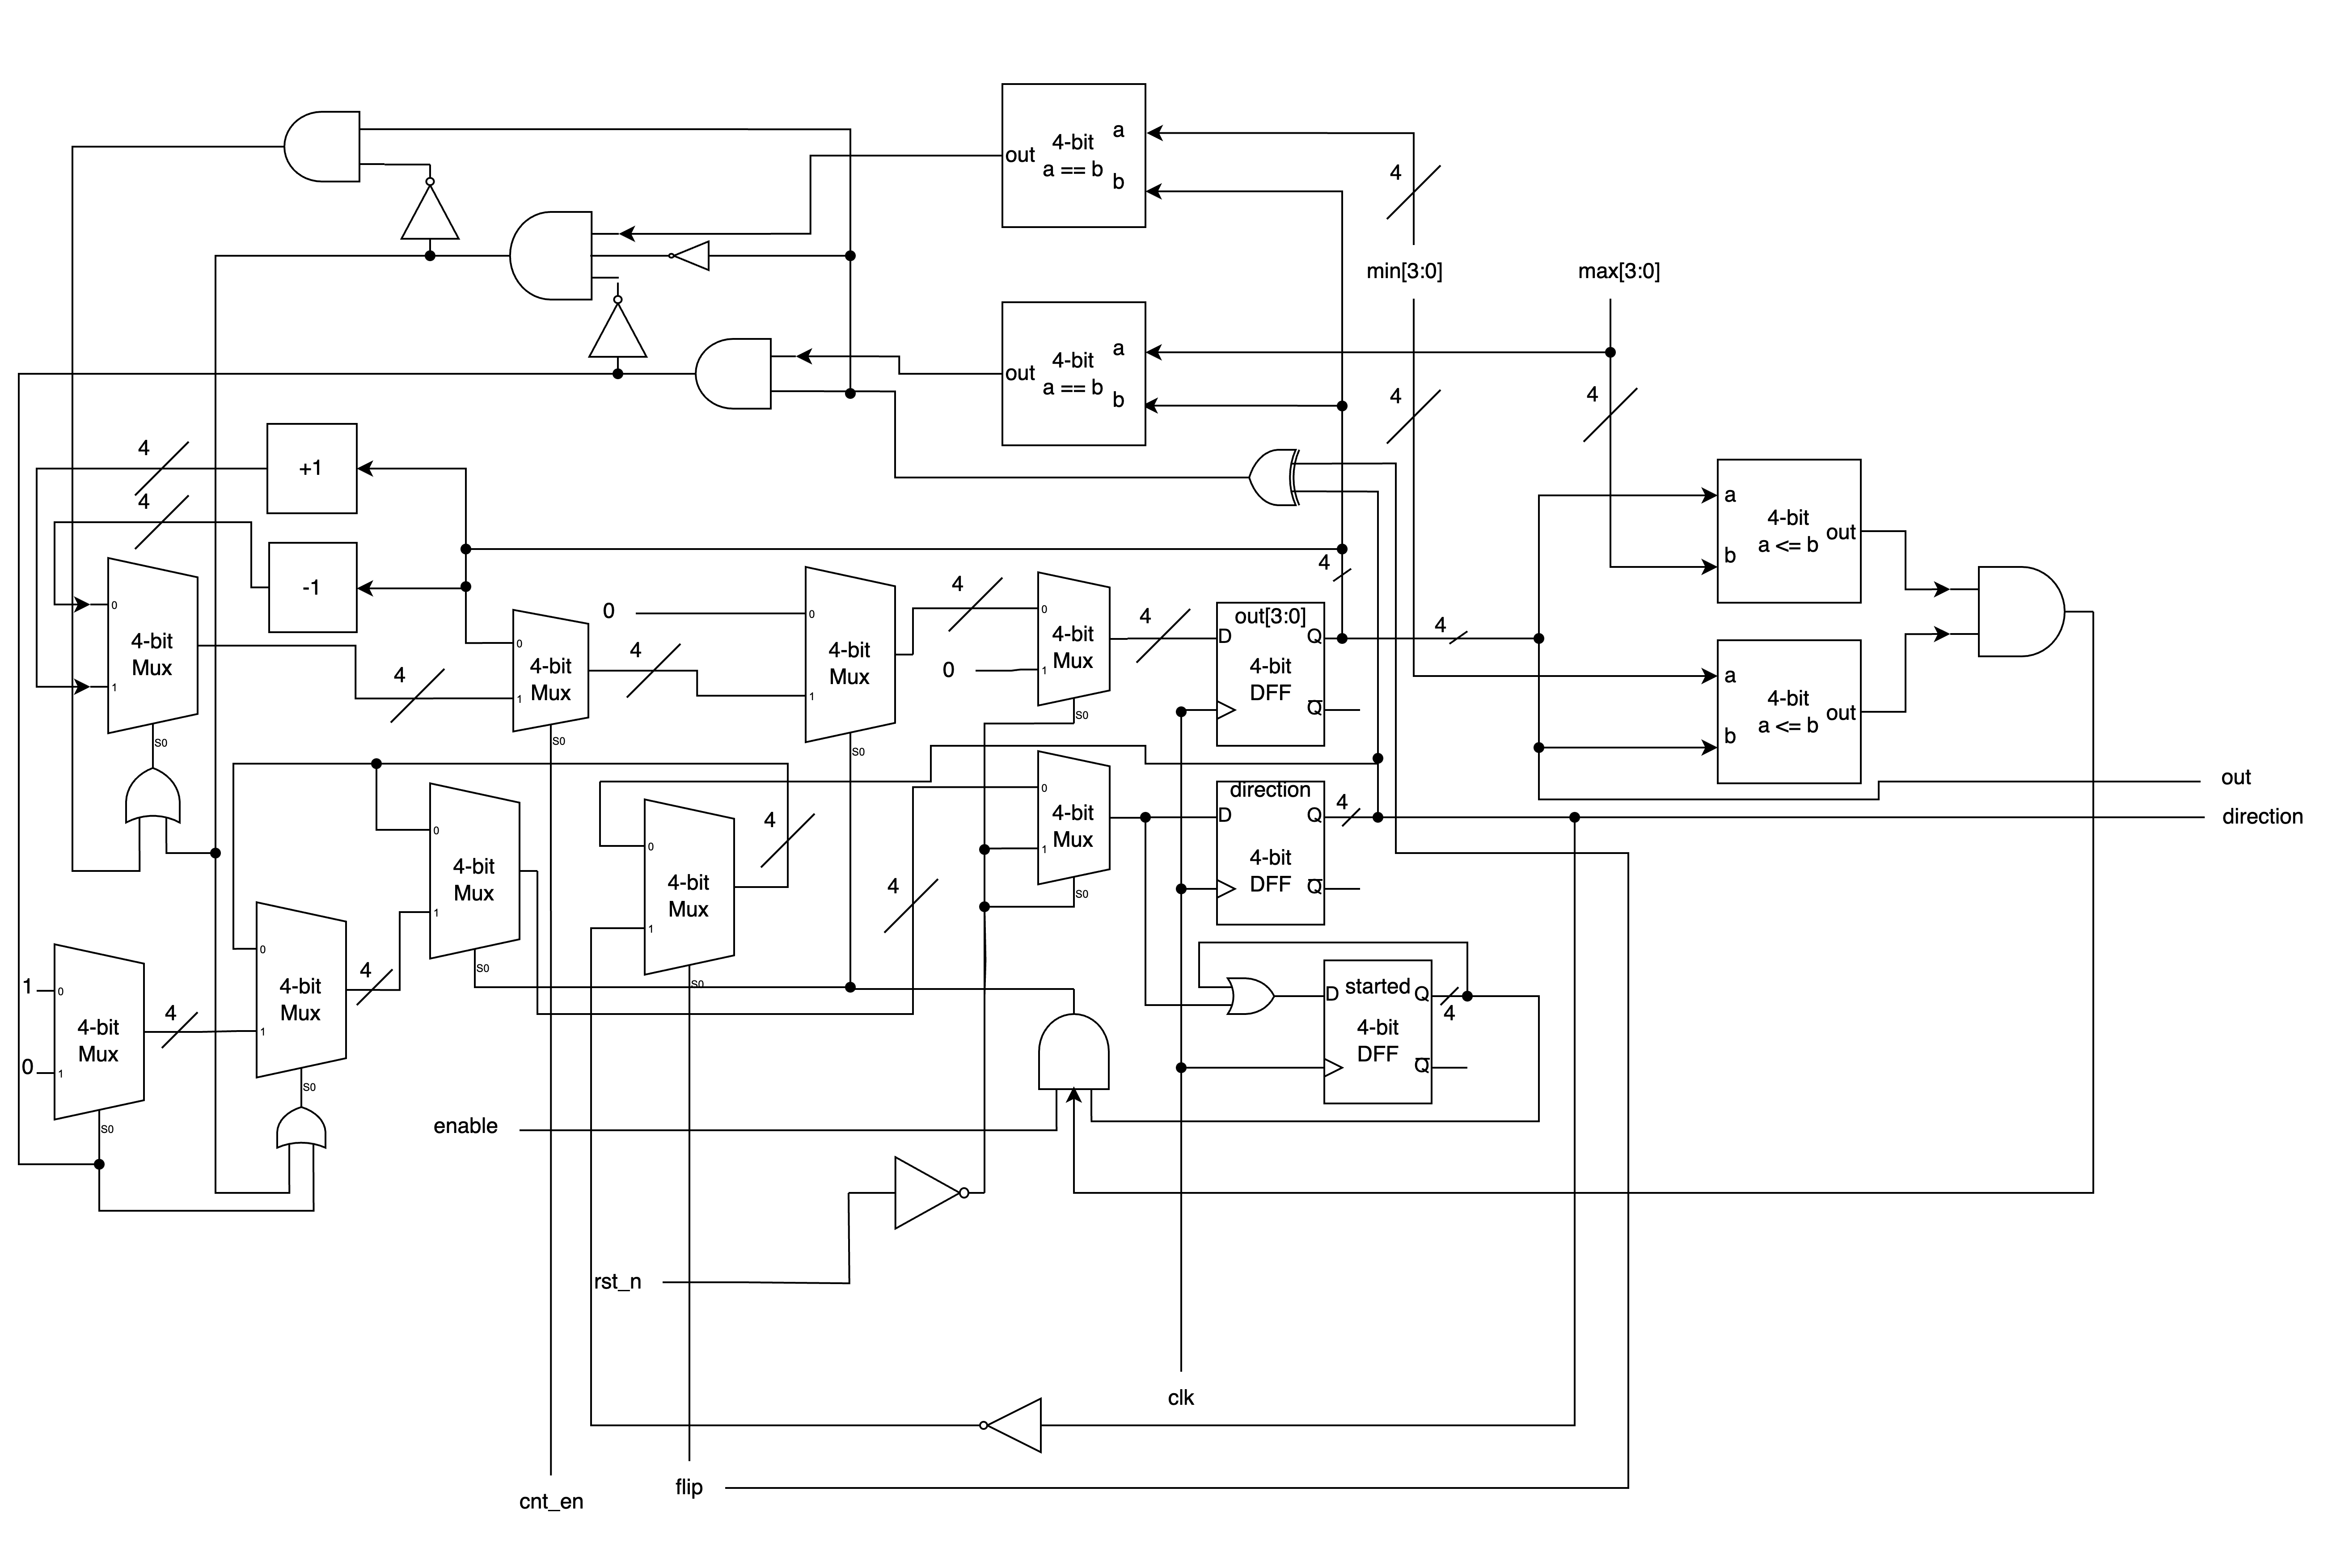
\includegraphics[width=\textwidth]{./img/FPGA.png}
  \caption{FPGA Counter}
  \label{fig:FPGA}
\end{figure}

\newpage

\subsection{debounce}
\subsubsection*{Implement}
首先要介紹 debounce,這是為了要避免按鈕會出現雜訊,導致沒有辦法成功讀到正確的訊號。\
\par
因為在 FPGA 上,clock 的時脈是 100MHz,因此按鈕按下的時候,會經過很多次 clock cycle。\
我們可以利用這個性質,判斷按鈕的訊號是不是連續好幾個 clock 都很穩定,\
這次使用的是四個 D-Flip-Flop,互相串接,並且在四個輸出都是 True 的時候才會輸出 True 訊號,\
這樣的做法可以確保訊號真實穩定經過了 4 個 clock cycle 以上。

\subsubsection*{Circuit}
\begin{figure}[!h]
  \centering
  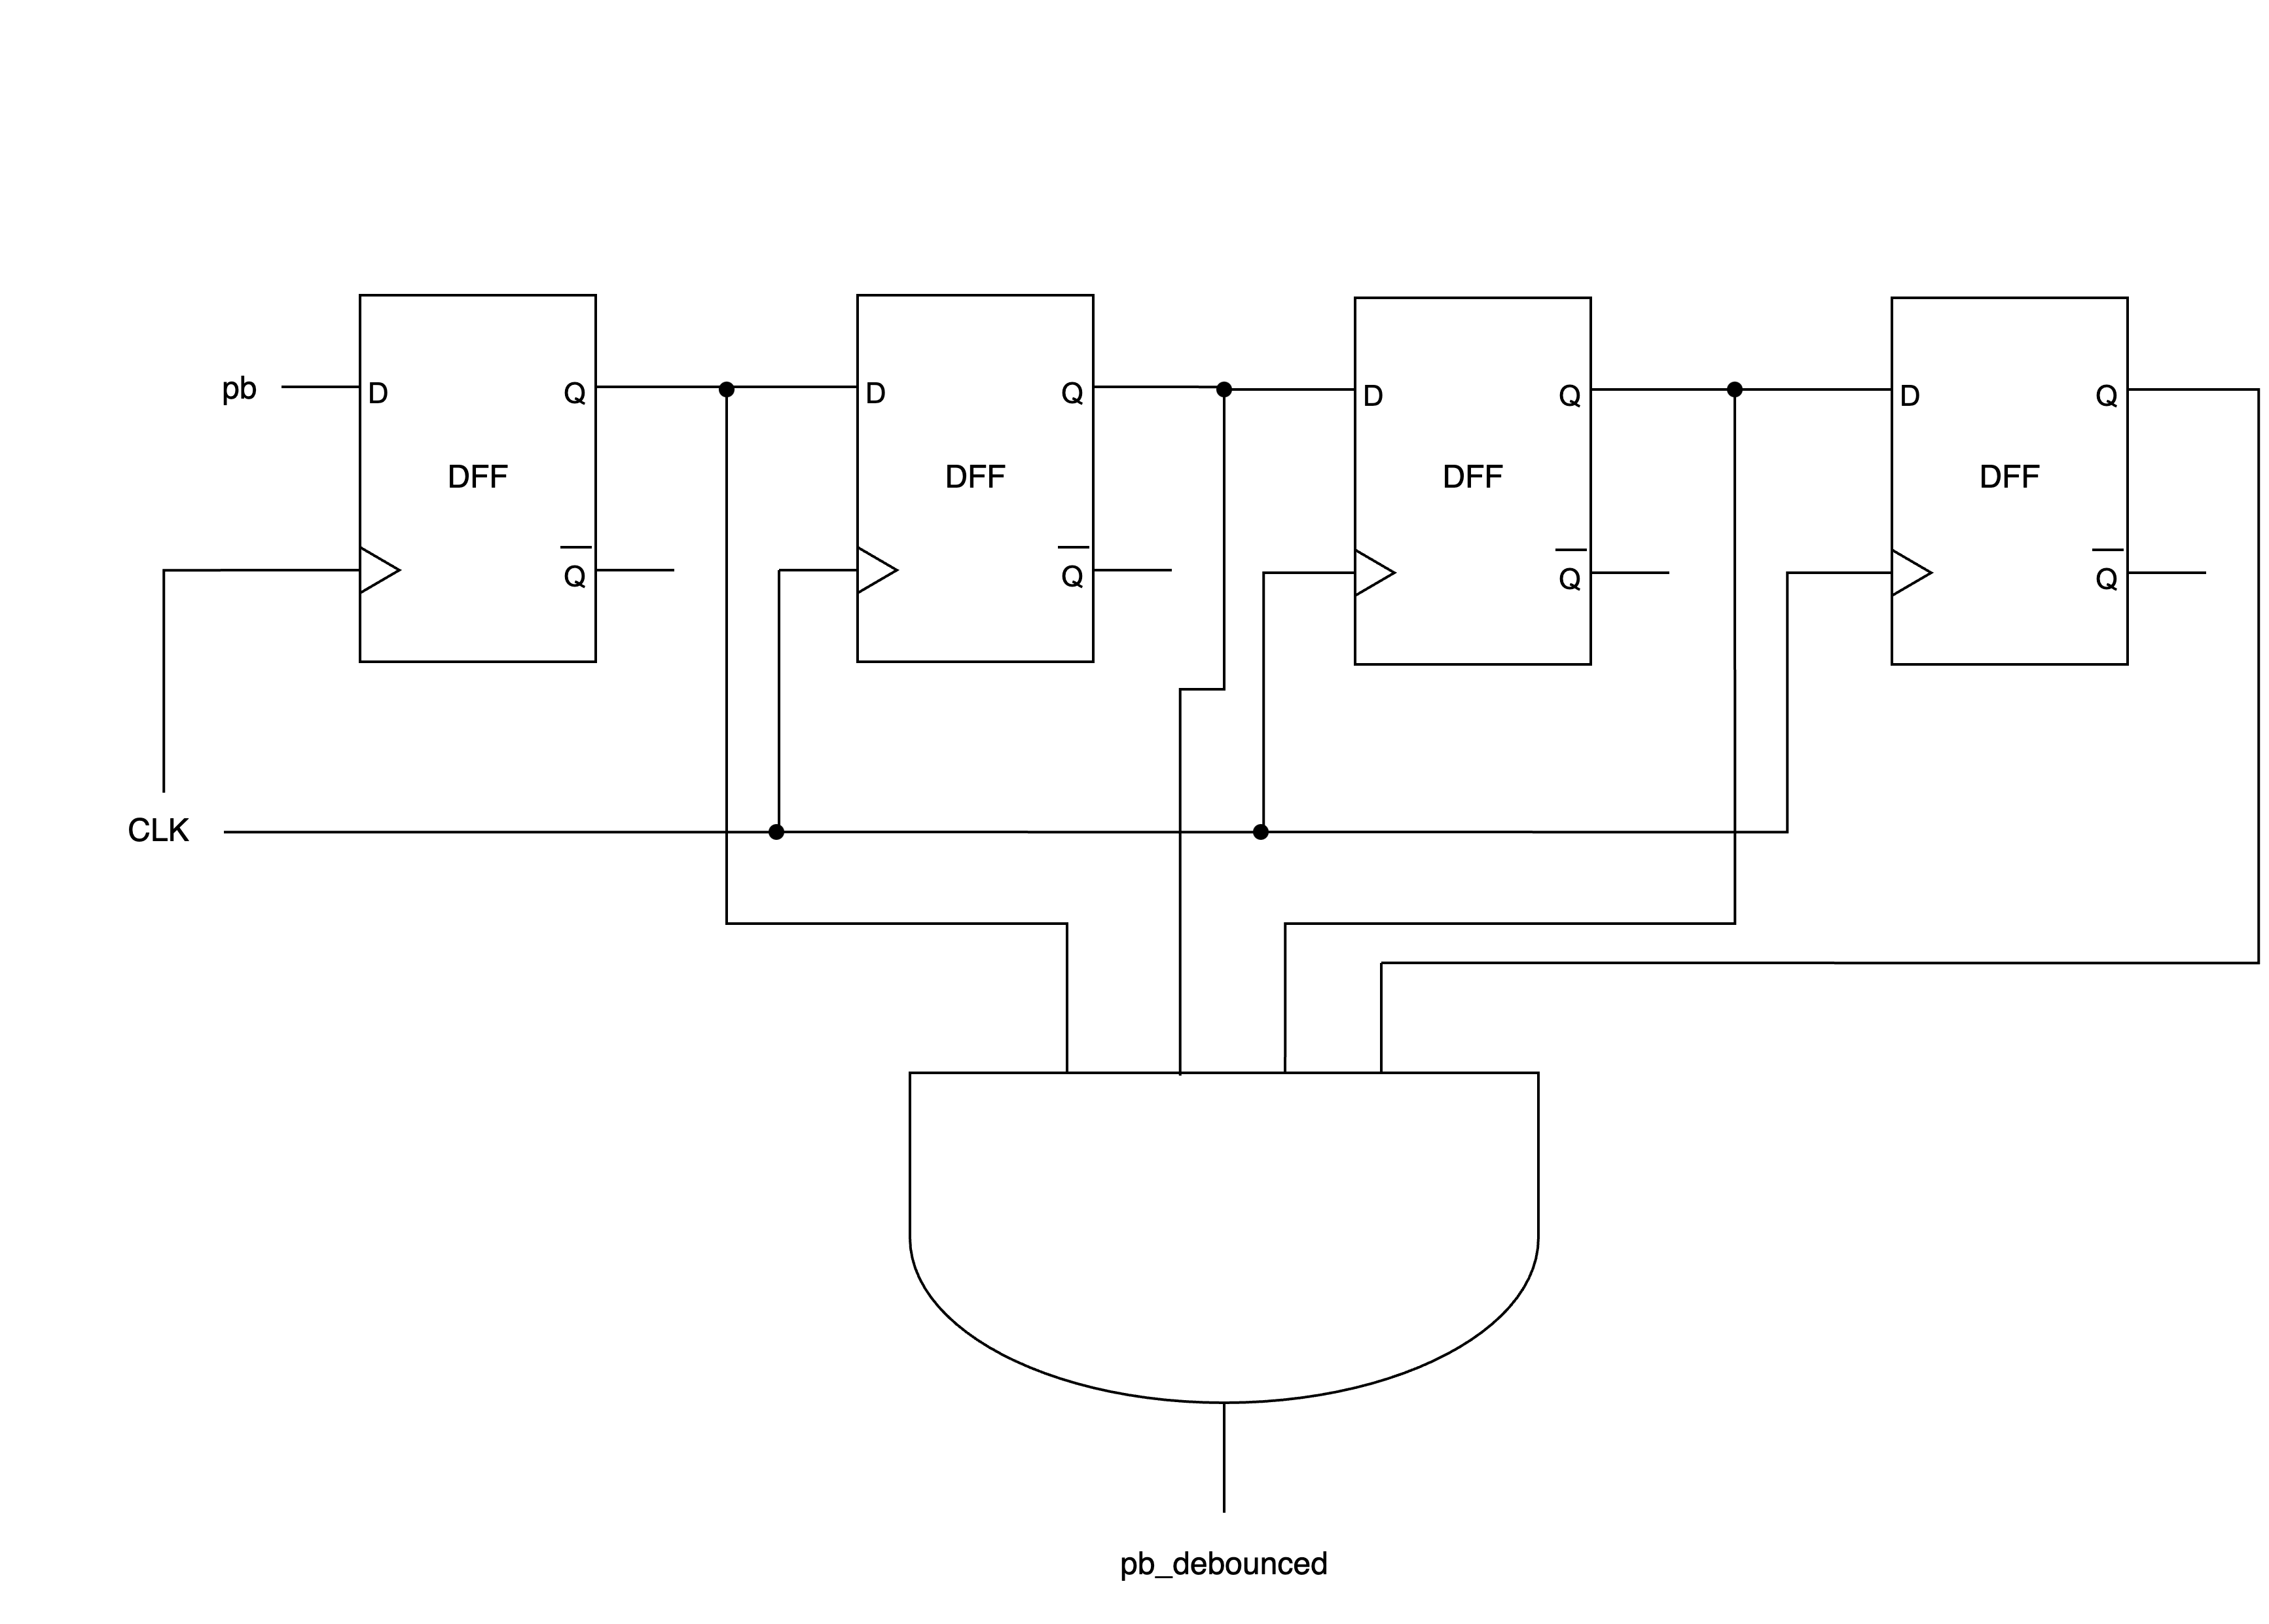
\includegraphics[width=\textwidth]{./img/Q5-Debounce.png}
  \caption{Debounce}
  \label{fig:debounce}
\end{figure}

\newpage

\subsection{One Pulse}
\subsubsection*{Implement}
接續上一個問題,由於按鈕按下會經過很多個 clock cycle,直接作為輸入的話會導致判定為多次輸入\
,因此需要一個 One Pulse 模組,讓按鈕在按下的時候只會輸出一次訊號。
\par
首先,利用 D-flip-flop 使得訊號延遲一單位,並將其反相。接著將其與原本的訊號做 AND 運算,\
就會產生一個只有一個 clock cycle 兩個都是 True 的訊號,最後再將其導向一個 D-Flip-Flop,\
最後的輸出就會是一個只有一個 clock cycle 是 True 的訊號,如下圖。

\begin{figure}[!h]
  \centering
  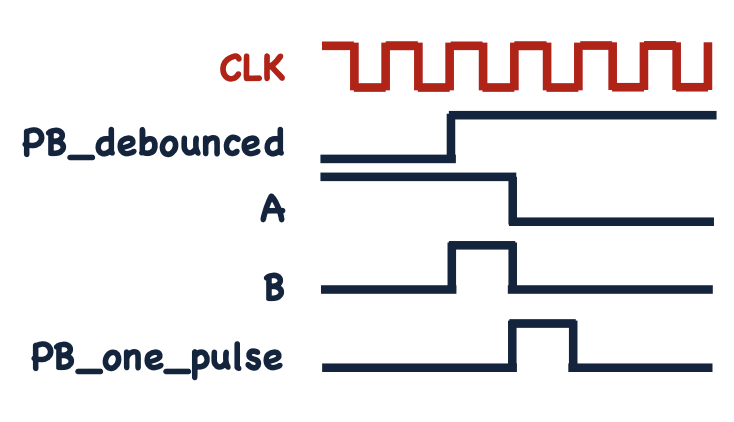
\includegraphics[width=0.5\textwidth]{./img/Q5-One-pulse-wave.png}
  \caption{One Pulse wave}
  \label{fig:one-pulse-wave}
\end{figure}


\subsubsection*{Circuit}
\begin{figure}[!h]
  \centering
  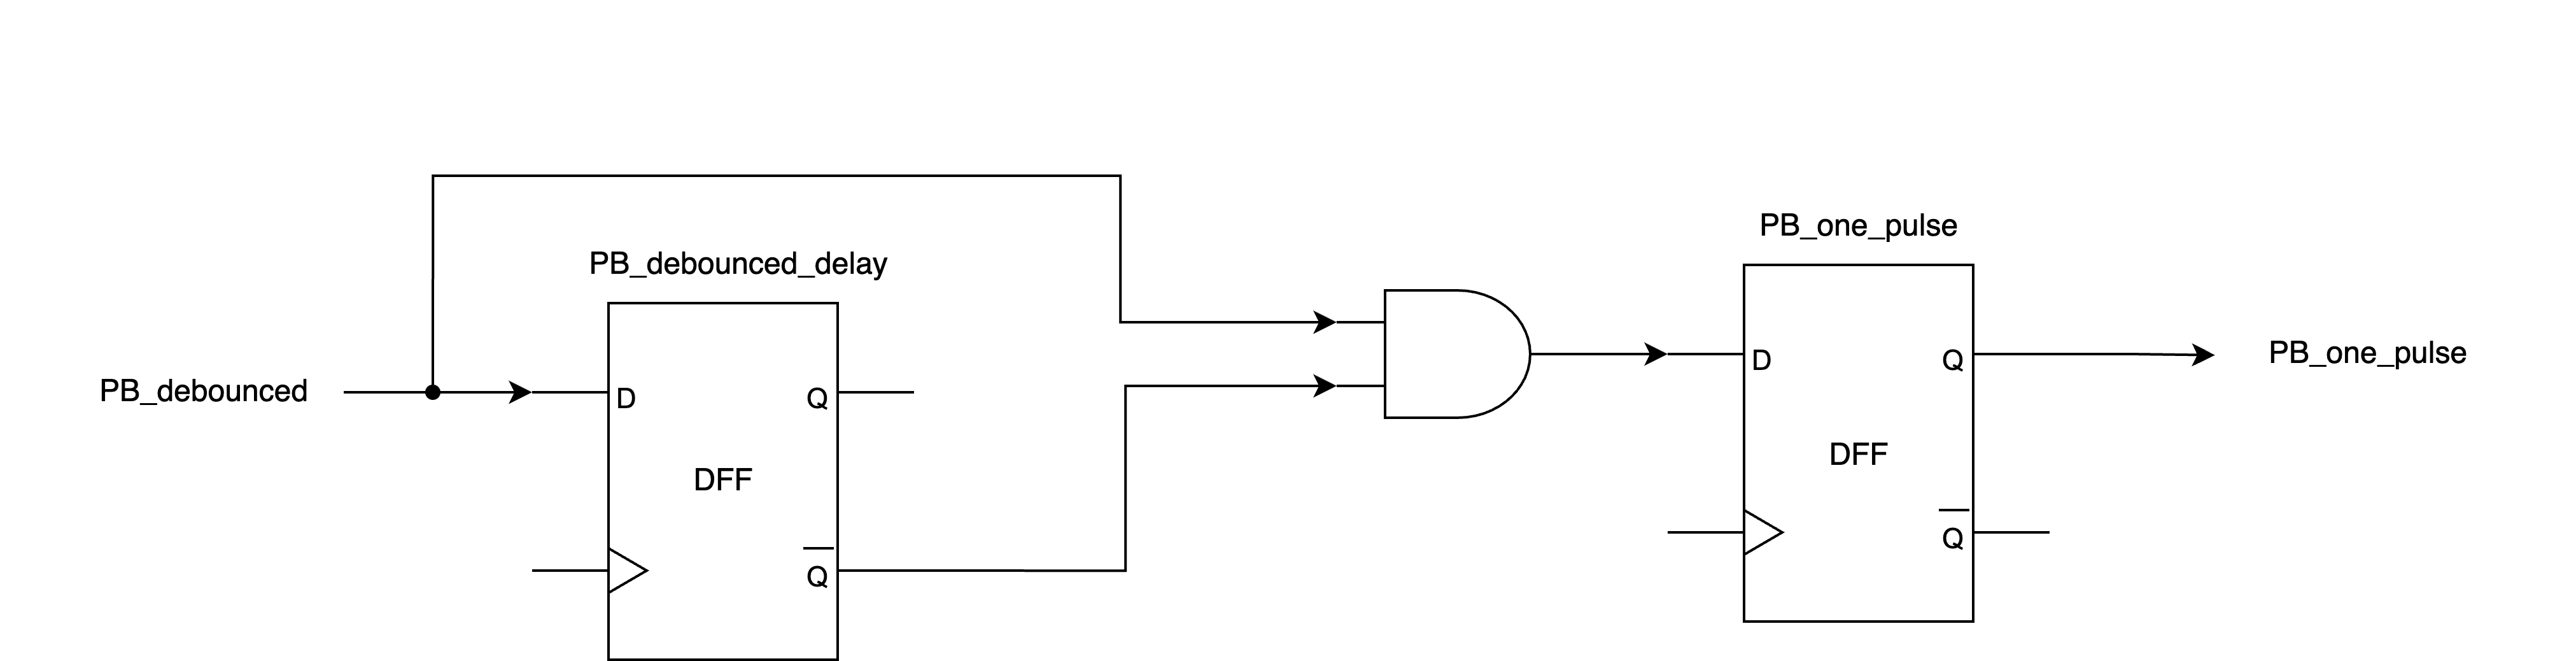
\includegraphics[width=\textwidth]{./img/Q5-One-pulse.png}
  \caption{One Pulse Circuit}
  \label{fig:one-pulse}
\end{figure}

\newpage

\subsection{Display Control}
由於 FPGA 上的頻率為 100MHZ,對於某些計算來說太快了,因此這邊先定義了一個 32-bit 的整數:$counter$,\
每 $33554432 (2^{24})$ 個 clock cycle 為一個循環用來控制 Counter 加減法的頻率,\
使得其頻率降到原本的 $\frac{1}{2^{24}}$。
\par
除此之外,我們取了這個整數的第 15, 16 個 bit,作為七段顯示器的切換頻率,使其能夠降到原始 clock 頻率的\
$\frac{1}{2^{15}}$
\par
接著是 Counter 的部分,我們在原來的基礎上加上了 $cnt\_en$ 這個參數,當 $counter$ 經過一個循環後,\
$cnt\_en$ 就會變成 True 一個 clock cycle,並進行加減法的操作。但如果中途有 flip, reset 的操作,\
就會直接改變輸出值,並且將 $counter$ 重設。
\par
Counter 算出數值後,接著要將輸出的數字 $digit$ 以及方向 $direction$ 輸出到七段顯示器上。\
首先是 $direction$,我們利用這個表達式算出了 $direction$ 與七段顯示器最右邊兩個單位的 $seg$ 值:
$$seg[0] = (direction == 1) ? \lnot(7'b0100011) : \lnot(7'b0011100)$$
$$seg[1] = (direction == 1) ? \lnot(7'b0011000) : \lnot(7'b0000011)$$

至於七段顯示器的部分,與上次的 Lab 類似,我們統計了 $digit = 0 \sim 9$ 的情況下,\
每一段所對應的布林表達式:
\begin{itemize}
  \item $A: out = nor(num[0], num[2], num[3],
  num[5], num[6], num[7], num[8], num[9])$
  \item $B: out = nor(num[0], num[1], num[2], num[3], num[4],
  num[7], num[8], num[9])$
  \item $C: out = nor(num[0], num[1], num[3], num[4],
  num[5], num[6], num[7], num[8], num[9])$
  \item $D: out = nor(num[0], num[2], num[3], 
  num[5], num[6], num[8])$
  \item $E: out = nor(num[0], num[2],
  num[6], num[8])$
  \item $F: out = nor(num[0], num[4],
        num[5], num[6], num[8], num[9])$
  \item $G: out = nor(num[2], num[3], num[4],
        num[5], num[6], num[8], num[9])$
\end{itemize}
\par

至於這些 $num[]$ 可以透過左移的方式產生:
$$num[0] = 1 << (digit >= 10 ? digit - 10 : digit)$$
$$num[1] = 1 << (digit >= 10)$$

得到每一段的 out 之後,就可以開始處理七段顯示器的輸出,\
由於輸出頻率是 FPGA 的 $\frac{1}{15}$,因此在任意時間下,\
要輸出的單位就是 $counter[16:15]$,利用這個性質,\
用以下的式子就可以成功的運算出七段顯示器的設定。
$$seg_out = seg[counter[16:15]]$$
$$an[0] = counter[16:15] != 0;$$
$$assign an[1] = counter[16:15] != 1;$$
$$assign an[2] = counter[16:15] != 2;$$
$$assign an[3] = counter[16:15] != 3;$$

\section{Other}
\subsection*{What we have learned}
\begin{enumerate}
  \item 記憶體:透過這次的實作,能夠了解到如果要實現讀寫 lock 的話要怎麼實作,\
  並將其應用到第三題的 Multi-Bank Memory 上。該題目呈現了硬體中大致上的記憶體架構,\
  以及電腦是如果透過分區來 lock 讀寫的機制。我想這也是為什麼我們在寫平行程式等需要大量讀寫演算法的時候,\
  會需要考慮 IO lock 的問題。
  \item Sequential Circuit:由於資料只會在 posedge 的時候改變,\
  會像是 pipeline 的形式,因此在思考如何設計的時候會更加不容易,\
  除了需要考慮到每經過一個 D-Flip-Flop,就會多一個 clock cycle 的延遲,\
  以及資料運算的設計方式,不能用平常在寫程式的變數來思考,必須帶入到一個以「狀態」為單位的思考模式。
  \item MUX 等工具的運用:之前寫程式或是 Gate Level 的時候,有時候會習慣直接將一個變數以一個 bool expression 來表示,\
  而不是使用 if 條件式,在寫程式的角度可能會覺得很簡潔有力,但是在畫電路圖的時候,\
  有時候反而會覺得可讀性降低,反而用 MUX 來處理分支會比較知道那個訊號的意義是什麼。\
  再加上有些語法本身不容易畫成電路圖,導致最後在畫的時候花了一些時間在修改及測試程式碼,\
  之後寫的時候應該要更多加注意這樣的程式,是否容易實現成電路。
  \item FPGA:上次 Lab 只有顯示一個單位(數字),所以不會有輪詢率的問題,\
  但這次需要顯示四個單位,因此需要讓他們以足夠高且合適的頻率輪流顯示,才能夠清楚地顯示,\
  這部分最簡單的方式就是直接用一個 counter,並除以一個數字來決定要經過幾個 clock cycle 才能夠換下一個單位。\
  但是硬體在除法以及 mod 的運算上特別麻煩,因此我後來想到以二進位的性質,直接存取某幾個 bit 或是左移,\
  只要除數都是 2 的冪次,就能直接實現除法以及 mod。
  
\end{enumerate}

\subsection*{分工}
\begin{itemize}
  \item 陳克盈:程式碼、報告
  \item 蔡明妡:電路圖
\end{itemize}



\end{document}


